\pdfoutput=1

%%
%% This is file `sample-tinyml.tex',
%% generated with the docstrip utility.
%%
%% The original source files were:
%%
%% samples.dtx  (with options: `tinyml')
%%
%% IMPORTANT NOTICE:
%%
%% For the copyright see the source file.
%%
%% Any modified versions of this file must be renamed
%% with new filenames distinct from sample-tinyml.tex.
%%
%% For distribution of the original source see the terms
%% for copying and modification in the file samples.dtx.
%%
%% This generated file may be distributed as long as the
%% original source files, as listed above, are part of the
%% same distribution. (The sources need not necessarily be
%% in the same archive or directory.)
%%
%% The first command in your LaTeX source must be the \documentclass command.
\documentclass[tinyml]{acmart}

%%
%% \BibTeX command to typeset BibTeX logo in the docs
\AtBeginDocument{%
  \providecommand\BibTeX{{%
    \normalfont B\kern-0.5em{\scshape i\kern-0.25em b}\kern-0.8em\TeX}}}

%% Rights management information.  This information is sent to you
%% when you complete the rights form.  These commands have SAMPLE
%% values in them; it is your responsibility as an author to replace
%% the commands and values with those provided to you when you
%% complete the rights form.
\setcopyright{rightsretained}
%\setcopyright{none}
\copyrightyear{2025}
\acmYear{2025}

%% These commands are for a PROCEEDINGS abstract or paper.
% \acmConference[Woodstock '18]{Woodstock '18: ACM Symposium on Neural
%   Gaze Detection}{June 03--05, 2018}{Woodstock, NY}

%%
%% end of the preamble, start of the body of the document source.

\settopmatter{printacmref=false}

\usepackage{threeparttable}
\usepackage{pgfplots}
\pgfplotsset{compat=1.18}
\usepackage{tikz}
\usepackage{amsmath}
\usepackage{cases}
\usepackage{subfig}
\usepackage{xcolor,colortbl}
\usepackage{multirow}
\usepackage{url}
\usepackage{IEEEtrantools}

\usetikzlibrary{arrows.meta,positioning,automata}
\usetikzlibrary{backgrounds,positioning,shapes.gates.logic.US}
\usetikzlibrary{shapes.geometric}

% heatmap
\usepackage{collcell}
\usepackage{enumitem}

\setlength{\textfloatsep}{5pt}
\setlength{\intextsep}{5pt}

\begin{document}

%%
%% The "title" command has an optional parameter,
%% allowing the author to define a "short title" to be used in page headers.
\title{\textit{ETHEREAL}: Energy-efficient and High-throughput Inference using Compressed Tsetlin Machine}

%%
%% The "author" command and its associated commands are used to define
%% the authors and their affiliations.
%% Of note is the shared affiliation of the first two authors, and the
%% "authornote" and "authornotemark" commands
%% used to denote shared contribution to the research.
\iffalse
\author{Ben Trovato}
\authornote{Both authors contributed equally to this research.}
\email{trovato@corporation.com}
\orcid{1234-5678-9012}
\author{G.K.M. Tobin}
\authornotemark[1]
\email{webmaster@marysville-ohio.com}
\affiliation{%
  \institution{Institute for Clarity in Documentation}
  \streetaddress{P.O. Box 1212}
  \city{Dublin}
  \state{Ohio}
  \country{USA}
  \postcode{43017-6221}
}
\fi

\author{Shengyu Duan}
\affiliation{%
  \institution{Newcastle University}
  \city{Newcastle upon Tyne}
  \country{UK}}
\email{shengyu.duan@newcastle.ac.uk}

\author{Rishad Shafik}
\affiliation{%
  \institution{Newcastle University}
  \city{Newcastle upon Tyne}
  \country{UK}}
\email{rishad.shafik@newcastle.ac.uk}

\author{Alex Yakovlev}
\affiliation{%
  \institution{Newcastle University}
  \city{Newcastle upon Tyne}
  \country{UK}}
\email{alex.yakovlev@newcastle.ac.uk}

%%
%% By default, the full list of authors will be used in the page
%% headers. Often, this list is too long, and will overlap
%% other information printed in the page headers. This command allows
%% the author to define a more concise list
%% of authors' names for this purpose.
%\renewcommand{\shortauthors}{Trovato and Tobin, et al.}

%%
%% The abstract is a short summary of the work to be presented in the
%% article.
\begin{abstract}
The Tsetlin Machine (TM) is a novel alternative to deep neural networks (DNNs). Unlike DNNs, which rely on multi-path arithmetic operations, a TM learns propositional logic patterns from data literals using Tsetlin automata. This fundamental shift from arithmetic to logic underpinning makes TM suitable for empowering new applications with low-cost implementations. 

In TM, literals are often included by both positive and negative clauses within the same class, canceling out their impact on individual class definitions. This property can be exploited to develop compressed TM models, enabling energy-efficient and high-throughput inferences for machine learning (ML) applications.

We introduce a training approach that incorporates excluded automata states to sparsify TM logic patterns in both positive and negative clauses. This exclusion is iterative, ensuring that highly class-correlated (and therefore significant) literals are retained in the compressed inference model, ETHEREAL, to maintain strong classification accuracy. Compared to standard TMs, ETHEREAL TM models can reduce model size by up to 87.54\%, with only a minor accuracy compromise. We validate the impact of this compression on eight real-world Tiny machine learning (TinyML) datasets against standard TM, equivalent Random Forest (RF) and Binarized Neural Network (BNN) on the STM32F746G-DISCO platform. Our results show that ETHEREAL TM models achieve over an order of magnitude reduction in inference time (resulting in higher throughput) and energy consumption compared to BNNs, while maintaining a significantly smaller memory footprint compared to RFs.
\end{abstract}

%%
%% Keywords. The author(s) should pick words that accurately describe
%% the work being presented. Separate the keywords with commas.
\keywords{Tsetlin Machine, Machine Learning, Model Compression, TinyML}


%%
%% This command processes the author and affiliation and title
%% information and builds the first part of the formatted document.
\maketitle

\section{Introduction} \label{sec:intro}
The ever increasing demand for deploying machine learning (ML) in low-energy, resource-constrained edge applications presents a significant challenge for deep neural network (DNN) implementations due to their high computational demands. This has led to efforts to identify alternative low-complexity ML algorithms. One such alternative is the Tsetlin Machine (TM), which is a novel ML algorithm that has been demonstrated with lower complexity than DNN, while achieving comparable accuracy across a range of ML datasets and exhibiting inherent interpretability \cite{granmo2018tsetlin}. A TM marks a fundamental shift from DNN by relying primarily on logic operations, which for example could outperform a multi-layer neural network (NN) in terms of accuracy \cite{tang2024adatm}, while eliminating hundreds of thousands of multiply-accumulate operations.

Figure \ref{fig:tm_structure} demonstrates a typical TM structure for supervised ML. The structure comprises three incremental processes:
\begin{itemize}
	\item [A.]\textit{Booleanization}: Before TM training and inference regimes, the input dataset is first expressed in the form of a set of literals, represented as Boolean data. These literals are derived through a data encoding process, known as Booleanization. A typical Booleanization process uses fixed or dynamic thresholds to generate Boolean literals as opposed to Binarized features from the raw data \cite{9923830}.
	\item [B.]\textit{Training}: Booleanized literals are given to a group of clauses, each learning a sub-pattern of some literals and performing AND operations to independently make a decision. Each clause learns these patterns through Tsetlin Automata (TAs), which decide whether a literal is included (above middle state) or excluded (below middle state), after a reinforcement learning process, see Section \ref{sec:learn} for further details. Half of all clauses have positive/negative polarity, capturing sub-patterns to support/oppose a classification. 
	\item [C.]\textit{Inference}: A binary classification is performed by a majority vote between the sum of outputs from positive and negative clauses. A multi-class classification requires as many pairs of positive-negative clauses as classes, where the overall classification is based on the one with the greatest class sum.
\end{itemize}

\definecolor{new_red}{rgb}{0.95,0.47,0.47}
\definecolor{new_green}{rgb}{0.85,0.98,0.77}

\definecolor{dark_red}{rgb}{0.78,0.28,0.34}
\definecolor{dark_green}{rgb}{0.09,0.30,0.28}

\tikzset{
	node distance = 0pt,
	BB/.style args={#1/#2/#3}{% Building Box, options
		draw, semithick, 
		font=\small\linespread{0.84}\selectfont, align=center, 
		minimum width=#1, minimum height=#2, text depth=0.25ex, 
		fill=#3, outer sep=0pt}
} % end of tikzset

\tikzset{
	sectors/.style n args={6}{minimum width=#1, minimum height=#2, 
		text depth=0.25ex, outer sep=0pt,
		append after command={\pgfextra{\let\LN\tikzlastnode
				\draw[fill=#3]  (\LN.west)  -| (\LN.north)
				{[rounded corners=3mm] -- (\LN.north west)}
				{[rounded corners=3mm] -- cycle}
				;
				
    			\draw[fill=#5]  (\LN.east)  -| (\LN.north)
				{[rounded corners=3mm] -- (\LN.north east)}
				[rounded corners=3mm] -- cycle;
				;
	} } }
}

\begin{figure}[!htb]
\vspace{-0.2cm}
\centering
\begin{tikzpicture}
[        GateCfg/.style={
	logic gate inputs={normal,normal},
	draw,
	thick,
	scale=1
	},
	cross/.style={path picture={ 
			\draw[black]
			(path picture bounding box.south east) -- (path picture bounding box.north west) (path picture bounding box.south west) -- (path picture bounding box.north east);
	}},
	scale=0.5, every node/.style={scale=0.5}
]
% clause M
\begin{scope}[xshift=1.45cm,yshift=2.5cm]
\draw[draw=black,fill=white] (-1.2,-7) rectangle ++(10.3,9);
\draw[draw=black,fill=black!30!white] (-1.2,1.5) rectangle ++(10.3,0.5) node[pos=.5] {\large{\textbf{Clause M}}};

\node[rotate=45] at (3.5,1.15) {\large{\textbf{...}}};

\draw[thick,arrows={-Triangle[]}] (9.1,-1.7) -- (9.6,-1.7);
\node[trapezium, draw, thick, minimum width=1cm, trapezium left angle=45, trapezium right angle=135, trapezium stretches=true, minimum height=0.8cm, fill=white] at (9.83,-1.9) {};
\node[rotate=45] at (9.83,-1.9) {$C_{M}$};

\draw[thick,arrows={-Triangle[]}] (10.23,-1.7) -- (11.4,-1.7);
\node [draw,thick,circle,cross,minimum width=0.4 cm,fill=white]() at (11.6,-1.7){};
\draw[arrows={-Triangle[]}] (11.6,-2.3) -- (11.6,-1.9);
\node[fill=blue!50!white] at (11.6,-2.4) {-1};

\draw[thick] (11.8,-1.7) -- (12.8,-1.7);
\draw[thick,arrows={-Triangle[]}] (12.8,-1.7) -- (12.1,-3.65);
\end{scope}

% clause M-1
\begin{scope}[xshift=1.15cm,yshift=1.8cm]
\draw[draw=black,fill=white] (-1.2,-7) rectangle ++(10.3,9);
\draw[draw=black,fill=black!30!white] (-1.2,1.5) rectangle ++(10.3,0.5) node[pos=.5] {\large{\textbf{Clause M-1}}};

\node[rotate=45] at (3.5,1.15) {\large{\textbf{...}}};

\draw[thick,arrows={-Triangle[]}] (9.1,-2) -- (9.5,-2);
\node[trapezium, draw, thick, minimum width=1cm, trapezium left angle=45, trapezium right angle=135, trapezium stretches=true, minimum height=0.8cm, fill=white] at (9.8,-2) {};
\node[rotate=45] at (9.8,-2) {\footnotesize{$C_{M-1}$}};
\node[rotate=70] at (9.5,-2.8) {\large{\textbf{...}}};

\draw[thick,arrows={-Triangle[]}] (10.1,-2) -- (11.1,-2);
\node [draw,thick,circle,cross,minimum width=0.4 cm,fill=white]() at (11.3,-2){};
\draw[arrows={-Triangle[]}] (11.3,-2.6) -- (11.3,-2.2);
\node[fill=yellow!50!white] at (11.3,-2.7) {+1};

\draw[thick] (11.5,-2) -- (11.8,-2);
\draw[thick,arrows={-Triangle[]}] (11.8,-2) -- (12,-3);
\end{scope}

% clause 2
\begin{scope}[xshift=0.3cm,yshift=0.7cm]
\draw[draw=black,fill=white] (-1.2,-7) rectangle ++(10.3,9);
\draw[draw=black,fill=black!30!white] (-1.2,1.5) rectangle ++(10.3,0.5) node[pos=.5] {\large{\textbf{Clause 2}}};

\draw[thick,arrows={-Triangle[]}] (9.1,-2.2) -- (9.9,-2.2);
\node[trapezium, draw, thick, minimum width=1cm, trapezium left angle=45, trapezium right angle=135, trapezium stretches=true, minimum height=0.8cm, fill=white] at (10.13,-2.4) {};
\node[rotate=45] at (10.13,-2.4) {$C_2$};

\draw[thick,arrows={-Triangle[]}] (10.55,-2.2) -- (11.4,-2.2);
\node [draw,thick,circle,cross,minimum width=0.4 cm,fill=white]() at (11.6,-2.2){};
\draw[arrows={-Triangle[]}] (11.6,-2.8) -- (11.6,-2.4);
\node[fill=blue!50!white] at (11.6,-2.9) {-1};

\draw[thick,fill=white] (13.1,-2.2) circle [radius=0.4] node () {\large{$\sum$}};
\draw[thick,arrows={-Triangle[]}] (11.8,-2.2) -- (12.7,-2.2);

% class sum
\node[trapezium, draw, thick, minimum width=1cm, trapezium left angle=45, trapezium right angle=135, trapezium stretches=true, minimum height=0.8cm, fill=white] at (14.3,-2.4) {};
\draw[thick,arrows={-Triangle[]}] (13.5,-2.2) -- (14.05,-2.2);
\node[] at (14.6,-1.7) {\large{\textbf{Class Sum}}};

\end{scope}

% TA states 1
\begin{scope}[xshift=0cm,yshift=0cm]
\draw[draw=black,fill=white] (-1.2,-7) rectangle ++(10.3,9);
\draw[draw=black,fill=black!30!white] (-1.2,1.5) rectangle ++(10.3,0.5) node[pos=.5] {\large{\textbf{Clause 1}}};
\node[] at (2.75,1.05) {\large{\textbf{Tsetlin Automata Team}}};

\node at (2.75,-0.7) [sectors= {72mm}{28mm}
{new_red}{}
{new_green}{}] {};

\draw[thick,fill=white] (0,0) circle [radius=0.3] node (s1) {1};
\draw[thick, arrows={-Stealth[reversed,reversed]},dashed] (-0.3,-0.2) to [out=230,in=160,looseness=4] (-0.3,0.2);
\draw[thick,fill=white] (1,0) circle [radius=0.3] node (s2) {2};
\draw[thick, arrows={-Stealth[reversed,reversed]}] (0,0.3) to [bend left=45] (1,0.3);
\draw[thick, arrows={Stealth[reversed,reversed]-},dashed] (0,-0.3) to [bend right=45] (1,-0.3);
\draw[thick,fill=white] (2.2,0) circle [radius=0.3] node (sn) {N};
\node[] at (1.6,0) {...};
\draw[thick, arrows={-Stealth[reversed,reversed]}] (1,0.3) to [bend left=35] (2.2,0.3);
\draw[thick, arrows={Stealth[reversed,reversed]-},dashed] (1,-0.3) to [bend right=35] (2.2,-0.3);

\draw[thick, arrows={-Stealth[reversed,reversed]}] (2.2,0.3) to [bend left=35] (3.3,0.3);
\draw[thick, arrows={Stealth[reversed,reversed]-},dashed] (2.2,-0.3) to [bend right=35] (3.3,-0.3);

\draw[thick,fill=white] (3.3,0) circle [radius=0.3] node (sn1) {\footnotesize{N+1}};
\draw[thick, arrows={-Stealth[reversed,reversed]}] (3.3,0.3) to [bend left=45] (4.3,0.3);
\draw[thick, arrows={Stealth[reversed,reversed]-},dashed] (3.3,-0.3) to [bend right=45] (4.3,-0.3);
\draw[thick,fill=white] (4.3,0) circle [radius=0.3] node (sn2) {};
\draw[draw=none,fill=black!25!white] (4.3,0) circle [radius=0.24] node () {\footnotesize{N+2}};
\node[] at (4.9,0) {...};
\draw[thick, arrows={-Stealth[reversed,reversed]}] (4.3,0.3) to [bend left=35] (5.5,0.3);
\draw[thick, arrows={Stealth[reversed,reversed]-},dashed] (4.3,-0.3) to [bend right=35] (5.5,-0.3);
\draw[thick,fill=white] (5.5,0) circle [radius=0.3] node (s2n) {2N};
\draw[thick, arrows={-Stealth[reversed,reversed]}] (5.8,0.2) to [out=30,in=330,looseness=4] (5.8,-0.2);

\draw[ultra thick, arrows={-Triangle[]}] (6.5,0) to (7.1,0);
\node[] at (7.4,0) {\large{$x_0$}};

\draw[ultra thick, arrows={-Triangle[]}] (-1.6,0) to (-1,0);
\node[] at (-2.2,0) {\large{$x_0$}};
\end{scope}

% TA states 2
\begin{scope}[xshift=0cm,yshift=-1.6cm]
\node at (2.75,-0.7) [sectors= {72mm}{28mm}
{new_red}{}
{new_green}{}] {};

\draw[thick,fill=white] (0,0) circle [radius=0.3] node (s1) {1};
\draw[thick, arrows={-Stealth[reversed,reversed]},dashed] (-0.3,-0.2) to [out=230,in=160,looseness=4] (-0.3,0.2);
\draw[thick,fill=white] (1,0) circle [radius=0.3] node (s2) {2};
\draw[draw=none,fill=black!25!white] (1,0) circle [radius=0.24] node () {2};
\draw[thick, arrows={-Stealth[reversed,reversed]}] (0,0.3) to [bend left=45] (1,0.3);
\draw[thick, arrows={Stealth[reversed,reversed]-},dashed] (0,-0.3) to [bend right=45] (1,-0.3);
\draw[thick,fill=white] (2.2,0) circle [radius=0.3] node (sn) {N};
\node[] at (1.6,0) {...};
\draw[thick, arrows={-Stealth[reversed,reversed]}] (1,0.3) to [bend left=35] (2.2,0.3);
\draw[thick, arrows={Stealth[reversed,reversed]-},dashed] (1,-0.3) to [bend right=35] (2.2,-0.3);

\draw[thick, arrows={-Stealth[reversed,reversed]}] (2.2,0.3) to [bend left=35] (3.3,0.3);
\draw[thick, arrows={Stealth[reversed,reversed]-},dashed] (2.2,-0.3) to [bend right=35] (3.3,-0.3);

\draw[thick,fill=white] (3.3,0) circle [radius=0.3] node (sn1) {\footnotesize{N+1}};
\draw[thick, arrows={-Stealth[reversed,reversed]}] (3.3,0.3) to [bend left=45] (4.3,0.3);
\draw[thick, arrows={Stealth[reversed,reversed]-},dashed] (3.3,-0.3) to [bend right=45] (4.3,-0.3);
\draw[thick,fill=white] (4.3,0) circle [radius=0.3] node (sn2) {\footnotesize{N+2}};
\node[] at (4.9,0) {...};
\draw[thick, arrows={-Stealth[reversed,reversed]}] (4.3,0.3) to [bend left=35] (5.5,0.3);
\draw[thick, arrows={Stealth[reversed,reversed]-},dashed] (4.3,-0.3) to [bend right=35] (5.5,-0.3);
\draw[thick,fill=white] (5.5,0) circle [radius=0.3] node (s2n) {2N};
\draw[thick, arrows={-Stealth[reversed,reversed]}] (5.8,0.2) to [out=30,in=330,looseness=4] (5.8,-0.2);

\draw[ultra thick, arrows={-Triangle[]}] (-1.6,0) to (-1,0);
\node[] at (-2.2,0) {\large{$\overline{x_0}$}};
\end{scope}

% TA states 3
\begin{scope}[xshift=0cm,yshift=-3.2cm]
\node at (2.75,-0.7) [sectors= {72mm}{28mm}
{new_red}{}
{new_green}{}] {};

\draw[thick,fill=white] (0,0) circle [radius=0.3] node (s1) {1};
\draw[thick, arrows={-Stealth[reversed,reversed]},dashed] (-0.3,-0.2) to [out=230,in=160,looseness=4] (-0.3,0.2);
\draw[thick, arrows={-Stealth[reversed,reversed]}] (0,0.3) to [bend left=45] (1,0.3);
\draw[thick,fill=white] (1,0) circle [radius=0.3] node (s2) {2};
\draw[thick, arrows={Stealth[reversed,reversed]-},dashed] (0,-0.3) to [bend right=45] (1,-0.3);
\draw[thick,fill=white] (2.2,0) circle [radius=0.3] node (sn) {};
\draw[draw=none,fill=black!25!white] (2.2,0) circle [radius=0.24] node () {N};
\node[] at (1.6,0) {...};
\draw[thick, arrows={-Stealth[reversed,reversed]}] (1,0.3) to [bend left=35] (2.2,0.3);
\draw[thick, arrows={Stealth[reversed,reversed]-},dashed] (1,-0.3) to [bend right=35] (2.2,-0.3);

\draw[thick, arrows={-Stealth[reversed,reversed]}] (2.2,0.3) to [bend left=35] (3.3,0.3);
\draw[thick, arrows={Stealth[reversed,reversed]-},dashed] (2.2,-0.3) to [bend right=35] (3.3,-0.3);

\draw[thick,fill=white] (3.3,0) circle [radius=0.3] node (sn1) {\footnotesize{N+1}};
\draw[thick, arrows={-Stealth[reversed,reversed]}] (3.3,0.3) to [bend left=45] (4.3,0.3);
\draw[thick, arrows={Stealth[reversed,reversed]-},dashed] (3.3,-0.3) to [bend right=45] (4.3,-0.3);
\draw[thick,fill=white] (4.3,0) circle [radius=0.3] node (sn2) {\footnotesize{N+2}};
\node[] at (4.9,0) {...};
\draw[thick, arrows={-Stealth[reversed,reversed]}] (4.3,0.3) to [bend left=35] (5.5,0.3);
\draw[thick, arrows={Stealth[reversed,reversed]-},dashed] (4.3,-0.3) to [bend right=35] (5.5,-0.3);
\draw[thick,fill=white] (5.5,0) circle [radius=0.3] node (s2n) {2N};
\draw[thick, arrows={-Stealth[reversed,reversed]}] (5.8,0.2) to [out=30,in=330,looseness=4] (5.8,-0.2);

\draw[ultra thick, arrows={-Triangle[]}] (-1.6,0) to (-1,0);
\node[] at (-2.2,0) {\large{$x_1$}};
\end{scope}

% TA states 4
\begin{scope}[xshift=0cm,yshift=-4.8cm]
\node at (2.75,-0.7) [sectors= {72mm}{28mm}
{new_red}{}
{new_green}{}] {};

\draw[thick,fill=white] (0,0) circle [radius=0.3] node (s1) {1};
\draw[thick, arrows={-Stealth[reversed,reversed]},dashed] (-0.3,-0.2) to [out=230,in=160,looseness=4] (-0.3,0.2);
\draw[thick,fill=white] (1,0) circle [radius=0.3] node (s2) {2};
\draw[thick, arrows={-Stealth[reversed,reversed]}] (0,0.3) to [bend left=45] (1,0.3);
\draw[thick, arrows={Stealth[reversed,reversed]-},dashed] (0,-0.3) to [bend right=45] (1,-0.3);
\draw[thick,fill=white] (2.2,0) circle [radius=0.3] node (sn) {N};
\node[] at (1.6,0) {...};
\draw[thick, arrows={-Stealth[reversed,reversed]}] (1,0.3) to [bend left=35] (2.2,0.3);
\draw[thick, arrows={Stealth[reversed,reversed]-},dashed] (1,-0.3) to [bend right=35] (2.2,-0.3);

\draw[thick, arrows={-Stealth[reversed,reversed]}] (2.2,0.3) to [bend left=35] (3.3,0.3);
\draw[thick, arrows={Stealth[reversed,reversed]-},dashed] (2.2,-0.3) to [bend right=35] (3.3,-0.3);

\draw[thick,fill=white] (3.3,0) circle [radius=0.3] node (sn1) {\footnotesize{N+1}};
\draw[thick, arrows={-Stealth[reversed,reversed]}] (3.3,0.3) to [bend left=45] (4.3,0.3);
\draw[thick, arrows={Stealth[reversed,reversed]-},dashed] (3.3,-0.3) to [bend right=45] (4.3,-0.3);
\draw[thick,fill=white] (4.3,0) circle [radius=0.3] node (sn2) {\footnotesize{N+2}};
\node[] at (4.9,0) {...};
\draw[thick, arrows={-Stealth[reversed,reversed]}] (4.3,0.3) to [bend left=35] (5.5,0.3);
\draw[thick, arrows={Stealth[reversed,reversed]-},dashed] (4.3,-0.3) to [bend right=35] (5.5,-0.3);
\draw[thick,fill=white] (5.5,0) circle [radius=0.3] node (s2n) {};
\draw[draw=none,fill=black!25!white] (5.5,0) circle [radius=0.24] node () {2N};
\draw[thick, arrows={-Stealth[reversed,reversed]}] (5.8,0.2) to [out=30,in=330,looseness=4] (5.8,-0.2);

\draw[ultra thick, arrows={-Triangle[]}] (6.5,0) to (7.1,0);
\node[] at (7.4,0) {\large{$\overline{x_1}$}};

\draw[ultra thick, arrows={-Triangle[]}] (-1.6,0) to (-1,0);
\node[] at (-2.2,0) {\large{$\overline{x_1}$}};

\node[] at (1.2,-1.05) {\textcolor{dark_red}{\large{\textbf{Exclude}}}};
\node[] at (4.5,-1.05) {\textcolor{dark_green}{\large{\textbf{Include}}}};

\begin{scope}[xshift=0.9cm,yshift=0cm]
\draw[thick,fill=white] (-0.8,-1.8) circle [radius=0.22] node () {};
\node[] at (-0.12,-1.8) {State};
\draw[thick,fill=white] (0.8,-1.8) circle [radius=0.22] node () {};
\draw[draw=none,fill=black!25!white] (0.8,-1.8) circle [radius=0.17] node () {};
\node[] at (1.95,-1.8) {Active state};
\draw[thick, arrows={-Stealth[reversed,reversed]}] (3.05,-1.8) to (3.55,-1.8);
\node[] at (4.3,-1.8) {Increment};
\draw[thick, arrows={-Stealth[reversed,reversed]},dashed] (5.3,-1.8) to (5.8,-1.8);
\node[] at (6.65,-1.8) {Decrement};
\end{scope}

\end{scope}

% clause output
\node[] at (-2.2,0.6) {\large{\textbf{Literal}}};
\draw[] (-2,0.2) -- ++(0.1,0) |- (-2,-5);
\draw[] (-2.45,0.2) -- ++(-0.1,0) |- (-2.45,-5);
\path (8.5,-2.5) node[and gate US,GateCfg] (AND1) {};
\draw[thick] (7.7,0) -- ++(0.1,0) |- (AND1.input 1); 
\draw[thick] (7.7,-4.8) -- ++(0.1,0) |- (AND1.input 2);
\node [draw,thick,circle,cross,minimum width=0.4 cm,fill=white]() at (11.3,-2.5){};
\draw[thick,arrows={-Triangle[]}] (AND1.output) -- (9.75,-2.5);

\node[trapezium, draw, thick, minimum width=1cm, trapezium left angle=45, trapezium right angle=135, trapezium stretches=true, minimum height=0.8cm, fill=white] at (10.1,-2.5) {};
\node[rotate=45] at (10.1,-2.5) {$C_1$};

\draw[thick,arrows={-Triangle[]}] (10.4,-2.5) -- (11.1,-2.5);
\draw[arrows={-Triangle[]}] (11.3,-3) -- (11.3,-2.7);
\node[fill=yellow!50!white] at (11.3,-3.2) {+1}; 

\node[] at (11.3,1.3) {\large{\textbf{Clause Output}}};

\draw[thick] (11.5,-2.5) -- (12.8,-2.5);
\draw[thick,arrows={-Triangle[]}] (12.8,-2.5) -- (13.2,-1.8);

\node[fill=yellow!50!white] at (11.3,-5) {+1};
\node[] at (12.9,-5) {Positive polarity};
\node[fill=blue!50!white] at (11.3,-5.6) {-1};
\node[] at (12.9,-5.6) {Negative polarity};
\end{tikzpicture}

\caption{The TM structure.}
\label{fig:tm_structure}
\Description[overall TM structure]

\vspace{-0.2cm}

\end{figure}


After training, TA array exhibits high sparsity; for example in the case of an MNIST dataset there are more than 99\% excludes. This property was leveraged to derive a compact model representation, REDRESS \cite{maheshwari2023redress}. The model only stores the information of includes as relative clauses and literal addressing. However, 
REDRESS, applied as a post-training compression, still follows the standard training process of the vanilla TM, resulting in a sparse form of training where the number of includes is not minimized, retaining less relevant or irrelevant context.
Reducing the number of includes is important in TMs, as their inherent sparse nature often incorporates literals with weak correlation to the target classes.  

It is possible to develop a more efficient TM by eliminating literals with weak correlations to a class, leading to minimal accuracy loss. 
{Though extensive research has been conducted on pruning weakly correlated features in DNNs, we emphasize that TM employs fundamentally different learning mechanism and data representation, and thus the pruning methods for DNNs are not applicable.}
In this work, we leverage the inherent interpretability of TM to identify weakly correlated literals, which are often included in both positive and negative clauses, due to their lack of strong association with a class. We propose a training approach to remove these literals, compressing TM models at the algorithm level, beyond REDRESS. This method, called \textbf{ETHEREAL}, enables \textbf{E}nergy-efficien\textbf{T}, \textbf{H}igh-throughput and accurate inf\textbf{E}rence through the practical implementation of a comp\textbf{RE}ssed tset\textbf{L}in m\textbf{A}chine. 

ETHEREAL introduces an additional exclusion process during training, to exclude literals shared by positive and negative clauses.
The exclusion is iteratively followed by standard training to restore important features. Results from eight real-world Tiny Machine Learning (TinyML) datasets show that ETHEREAL can realize up to an 87.54\% reduction in model size with a maximum accuracy loss of only 3.38\%, compared to a vanilla TM \cite{granmo2018tsetlin}. In some cases, accuracy even improves by eliminating some features that contribute noise. We use STM32F746G-DISCO micro-controller as the platform to implement ETHEREAL alongside REDRESS TM \cite{maheshwari2023redress}, a Random Forest (RF) and a Binarized Neural Network (BNN) \cite{courbariaux2016binarized, geiger2020larq}. The TM implementations can provide up to an order of magnitude reduction in inference time and energy compared to BNN, and 7$\times$ lower memory footprints than RF, while giving comparable accuracy. ETHEREAL further improves these design metrics, commensurate with the model size reductions achieved over REDRESS TMs. 

In this paper, we make the following key \textbf{\textit{contributions}}:
\begin{itemize}
	\item Empirical evidence revealing the inefficiency of vanilla TM in including less correlated (and thereby insignificant) literals.
	\item A training approach with additional exclusion, effectively compressing TM model and ensuring high accuracy.
	\item Validation with TinyML benchmarks on STM32 micro-controller, validating improved throughput, energy and memory usage produced by ETHEREAL. 
\end{itemize}

%We describe the TM learning process in Section \ref{sec:learn}. The ETHEREAL model compression method is introduced and evaluated in Sections \ref{sec:ethereal} and \ref{sec:eva}, respectively. We conclude our work in Section \ref{sec:conc}.

\section{TM Learning Dynamics} \label{sec:learn}
A TM is trained to capture the sub-pattern supporting or opposing a proposition by adjusting the TA states, which determine inclusion or exclusion of literals, driven by Type I and Type II feedback.

Figure \ref{fig:tm_feedbacks} explains the conditions under which each type of feedback is initiated. For a TA with 2N states, all TA states are initially set to either N or N+1 at random ($i.e.$, near the confusion state). During training, feedback is probabilistically activated for each datapoint; each specific type of feedback as well as the TAs being reinforced are determined by the training outcomes at the class and clause levels. 
%In Figure \ref{fig:tm_feedbacks}, $y$ indicates the label of a sample: for binary classification, $y$=1 or 0 suggests the sample belongs to the class or not, respectively; for multiclass classification and a TM for a certain class, $y$=1 or 0 suggests the sample belongs to the class or any other classes, respectively. 
%At a datapoint, each clause independently receives its feedback, the type of which is determined by both $y$ and the clause polarity: 
%\todo{This line repeats what you said earlier with a bit more specificity -- keep one; you actually repeat again in the following paragraph}
Type I/II feedback is activated for all positive/negative clauses when $y$=1, while an opposite reaction occurs when $y$=0.

\begin{figure}[!htb]
\centering

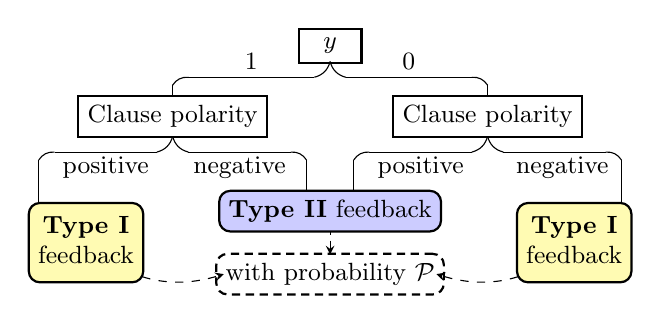
\begin{tikzpicture}[font=\small]
\node [draw, thick, shape=rectangle, minimum width=0.8cm] at (0,-0.3) {$y$};
\draw []  (0,-0.5) to [bend left] (-0.2,-0.7);
\draw [] (-0.2,-0.7) -- (-1.8,-0.7);
\node[] at (-1,-0.5) {1};
\draw []  (-1.8,-0.7) to [bend right] (-2,-0.8);
\draw [] (-2,-0.8) -- (-2,-1.25);
\draw []  (0,-0.5) to [bend right] (0.2,-0.7);
\draw [] (0.2,-0.7) -- (1.8,-0.7);
\node[] at (1,-0.5) {0};
\draw []  (1.8,-0.7) to [bend left] (2,-0.8);
\draw [] (2,-0.8) -- (2,-1.25);

\draw []  (-2,-1.45) to [bend left] (-2.2,-1.65);
\draw [] (-2.2,-1.65) -- (-3.5,-1.65);
\node[] at (-2.85,-1.85) {positive};
\draw[] (-3.5,-1.65) to [bend right] (-3.7,-1.75);
\draw[] (-3.7,-1.75) -- (-3.7,-3);
\draw []  (-2,-1.45) to [bend right] (-1.8,-1.65);
\draw [] (-1.8,-1.65) -- (-0.5,-1.65);
\node[] at (-1.15,-1.85) {negative};
\draw[] (-0.5,-1.65) to [bend left] (-0.3,-1.75);
\draw[] (-0.3,-1.75) -- (-0.3,-2.6);
\node [draw, thick, shape=rectangle, minimum width=0.8cm,fill=white] at (-2,-1.2) {Clause polarity};

\draw [-stealth,dashed]  (-3.1,-2.8) to [bend right] (-1.35,-3.2);

\node [draw, thick, shape=rectangle, minimum width=0.8cm, rounded corners, fill=yellow!30!white] at (-3.1,-2.8) {\begin{tabular}[c]{@{}c@{}} \textbf{Type I} \\ feedback \end{tabular}};

\draw []  (2,-1.45) to [bend left] (1.8,-1.65);
\draw [] (1.8,-1.65) -- (0.5,-1.65);
\node[] at (1.15,-1.85) {positive};
\draw[] (0.5,-1.65) to [bend right] (0.3,-1.75);
\draw[] (0.3,-1.75) -- (0.3,-2.6);
\draw []  (2,-1.45) to [bend right] (2.2,-1.65);
\draw [] (2.2,-1.65) -- (3.5,-1.65);
\node[] at (2.95,-1.85) {negative};
\draw[] (3.5,-1.65) to [bend left] (3.7,-1.75);
\draw[] (3.7,-1.75) -- (3.7,-2.6);
\node [draw, thick, shape=rectangle, minimum width=0.8cm,fill=white] at (2,-1.2) {Clause polarity};

\draw [-stealth, dashed]  (3.1,-2.8) to [bend left] (1.35,-3.2);

\node [draw, thick, shape=rectangle, minimum width=0.8cm, rounded corners, fill=yellow!30!white] at (3.1,-2.8) {\begin{tabular}[c]{@{}c@{}} \textbf{Type I}  \\ feedback \end{tabular}};

\draw [-stealth, densely dashed] (0,-2.6) -- (0,-2.95);

\node [draw, thick, shape=rectangle, minimum width=0.8cm, rounded corners, fill=blue!20!white] at (0,-2.4) {\textbf{Type II} feedback};

\node [draw, densely dashed, thick, shape=rectangle, minimum width=0.8cm, rounded corners] at (0,-3.2) {with probability $\mathcal{P}$};

\end{tikzpicture}

\caption{TM feedback procedure, independently performed for each clause. For binary classification, $y$=1 or 0 suggests the sample belongs to the class or not, respectively; for multiclass classification and a TM for a certain class, $y$=1 or 0 suggests the sample belongs to the class or other classes, respectively.}
\label{fig:tm_feedbacks}

\Description[overall TM feedback]

\end{figure}


Figure \ref{fig:tm_feedbacks} shows both types of feedback are triggered with probability $\mathcal{P}$, determined by a hyperparameter $T$, as in (\ref{eq:feedback_prob}):
\vspace{-0.2cm}
\begin{IEEEeqnarray}{rCl}
	\mathcal{P} =\dfrac{T+(-1)^y\times\textrm{clip}(\sum\limits_{j=1}^{M} p_j C_j, -T, T)}{2T}
	\label{eq:feedback_prob}
\end{IEEEeqnarray}
where $M$ is the number of clauses; $p_j$ and $C_j$ are the polarity and output, respectively, for a specific clause. According to (\ref{eq:feedback_prob}), the farther the class sum is from $T$/$-T$ when $y$=1/0, the more likely the feedback is triggered, potentially calibrating more clauses to cast correct votes. On the other hand, feedback is withheld if the class sum becomes greater/smaller than $T$/$-T$, when $y$=1/0. Therefore, $T$ reveals the confidence in distinguishing between different classes. 

Figure \ref{fig:type_i_ii} illustrates the mechanism of both types of feedback.
%In Type I feedback (Figure \ref{fig:type_i_ii} (a)), the TA state of a literal tends to increase, if the literal for the current training sample is `1' and the clause with positive/negative polarity manages to support for the fact that $y$=1/0 by producing the clause output as `1'. 
%Thus, in general, a clause that correctly produces the output is likely to include more literals equaling `1' at the datapoint, through Type I feedback. 
In Type I feedback (Figure \ref{fig:type_i_ii} (a)), a clause that correctly supports or opposes the class (by producing an output of `1') is likely to include more literals that equal `1' at the datapoint.
%\todo{avoid potentially -- use probabilistically or don't use at all.}
This enables it to continue making the right decision by using a more fine-grained sub-pattern. On the other hand, the TA state of a literal equal to `0' is decreased to prevent it from overturning the correct output. 

Finally, a clause that fails to support the correct class (by producing an output of `0') may cause a false negative.
As a result, all TA of the clause are penalized by decreasing their states. 
In other words, Type I feedback combats false negatives by denying established sub-patterns and regenerating them in later learning process.

\definecolor{new_red}{rgb}{0.95,0.47,0.47}
\definecolor{new_green}{rgb}{0.85,0.98,0.77}

\begin{figure}[!htb]
\vspace{-0.5cm}
\centering
\subfloat[]{
\begin{tikzpicture}[font=\small]
\node [draw=none, shape=rectangle, minimum width=0.8cm, rounded corners, fill=yellow!30!white] at (0,0.6) {\textbf{Type I} Feedback};

\draw []  (0,-0.25) to [bend left] (-0.2,-0.45);
\draw [] (-0.2,-0.45) -- (-1.1,-0.45);
\node[] at (-0.65,-0.6) {1};
\draw []  (-1.1,-0.45) to [bend right] (-1.3,-0.55);
\draw [->] (-1.3,-0.55) -- (-1.3,-0.95);

\draw []  (0,-0.25) to [bend right] (0.2,-0.45);
\draw [] (0.2,-0.45) -- (1.1,-0.45);
\node[] at (0.65,-0.6) {0};
\draw []  (1.1,-0.45) to [bend left] (1.3,-0.55);
\draw [->] (1.3,-0.55) -- (1.3,-2.15);
\node [draw, thick, shape=rectangle, minimum width=0.8cm, fill=white] at (0,0) {Clause output};

\node [draw, thick, shape=rectangle, minimum width=0.8cm] at (-1.3,-1.18) {Literal};
\draw[->] (-1.3,-1.4) -- (-1.3,-2.15);
\node[] at (-1.45,-1.775) {1};
\draw[] (-1.3,-1.4) to [bend right] (-1.1,-1.6);
\draw[] (-1.1,-1.6) -- (1.1,-1.6);
\draw[] (1.1,-1.6) to [bend left] (1.3,-1.7);
\node[] at (0,-1.775) {0};

\node [draw, thick, shape=rectangle, minimum width=0.8cm, rounded corners, fill=new_green] at (-1.35,-2.8) {\begin{tabular}[c]{@{}c@{}} TA state \\ \textbf{increments} with \\ probability $\frac{s-1}{s}$ \end{tabular}};

\node [draw, thick, shape=rectangle, minimum width=0.8cm, rounded corners, fill=new_red!50!white] at (1.35,-2.8) {\begin{tabular}[c]{@{}c@{}} TA state \\ \textbf{decrements} with \\ probability $\frac{1}{s}$ \end{tabular}};

\end{tikzpicture}
}
\hspace{0.2cm}
\subfloat[]{
\begin{tikzpicture}[font=\small]
\node [draw=none, shape=rectangle, minimum width=0.8cm, rounded corners, fill=blue!20!white] at (0,0.6) {\textbf{Type II} Feedback};

\draw [->]  (0,-1.4) -- (0,-2.15);
\node[] at (-0.15,-1.775) {0};
\node [draw, thick, shape=rectangle, minimum width=0.8cm, fill=white] at (0,0) {Clause output};
	
\draw [->]  (0,-0.25) -- (0,-0.95);
\node[] at (-0.15,-0.6) {1};
\node [draw, thick, shape=rectangle, minimum width=0.8cm,fill=white] at (0,-1.2) {Literal};

\node [draw, thick, shape=rectangle, minimum width=2cm, minimum height=1.32cm, rounded corners, fill=new_green] at (0,-2.8) {\begin{tabular}[c]{@{}c@{}} TA state \\ \textbf{increments} \end{tabular}};
	
\end{tikzpicture}
}
\vspace{-0.2cm}
\caption{(a) Type I and (b) Type II feedback, where TA state remains unchanged for any other cases.}
\label{fig:type_i_ii}

\Description[Type I/II feedback]

\end{figure}


The probability of changing a TA state is determined by another hyperparameter, $s$, which indicates the probability of including a literal. The larger the value of $s$, the more/less likely a literal is to be included/excluded through Type I feedback. So far, the optimal values for both $T$ and $s$ are determined based on extensive trials aimed at achieving optimal accuracy~\cite{maheshwari2023redress, tarasyuk2023systematic}. 

If a clause incorrectly supports a class proposition, a false positive may occur. For instance, a positive/negative clause output is `1', when $y$=0/1. False positives are minimized by Type II feedback (Figure \ref{fig:type_i_ii} (b)). This type of feedback increases the TA states for the literals equaling `0', which potentially modifies the incorrect clause output of `1'. The TA states of a clause with output as `0' keeps unchanged, to avoid being trapped by local minima.

\section{ETHEREAL Model Compression} \label{sec:ethereal} 
%This section presents evidence of inefficiency in vanilla TM due to the inclusion of insignificant literals based on a case study, followed by the ETHEREAL to address this issue.
\subsection{Literal Significance in Learning Dynamics}
The TM feedback mechanism given in Figure \ref{fig:type_i_ii}
ensures faster convergence during the training regime, through the interactions between both types of feedback. 
In addition, accuracy generally improves as more literals are included to capture fine-grained sub-patterns, as described in Section \ref{sec:learn}. However, this training process overlooks the significance or the correlation of individual literals to the target class. For example, a literal that consistently equals `1' does not provide useful information for classification, yet it can still be included in many clauses without adversely affecting accuracy.
%Nevertheless, as the training proceeds, a TM always keeps expanding by including more literals. This is because: 1) it is only possible to exclude a literal from a clause through Type I feedback, and 2) in Type I feedback, the probability of increasing a TA state will be greater than that of decreasing it, if $s$ is greater than 2, which is unfortunately the case for nearly all reported TM models with good accuracy.

We conduct an exploratory experiment to demonstrate how a TM model expands during training. In our experiment, the TM is trained to classify MNIST handwritten digits~\cite{deng2012mnist}, chosen as a case study for its simplicity in visualizing such an image classification task for our later analysis. We set the number of clauses per class, $T$ and $s$ to 100, 10 and 3, respectively, and Booleanize the dataset by applying a threshold of 75 to all grayscale values. Figure \ref{fig:TM_acc_size} shows resulting test accuracy and model size. As can be seen, the accuracy tends to increase with more training epochs, which is accompanied by a large increment on number of includes. This trend of model expansion is seen to hold across datasets and hyperparameters, as more TAs are included through random selection of automata reinforcements through $s$ and $T$ parameters explained above.


% \section{With what \emph{data}?}\label{sec:data}
\section{How do we \emph{train models}?}\label{sec:model_training}

% Which scales? How? 
%  - [DONE] Too small may not hold
%  - [DONE] number of models can affect confidence intervals
%  - [DONE] counting size also matters data (tokens vs bits) and flop counts kaplan vs hoffman CITE; non-embedding vs embedding 
%  - DITCH? how you scale architecture matters; for eg - clark shows scaling N and E is needed to separate; enc and decoder scaling can be different for architectures; in the 
%  - [DONE] 6ND is a common approximation - does not hold for very long context (these days 128k to 1M)


In order to fit a scaling law, one needs to train a range of models across multiple orders of magnitude in model size and/or dataset size. Researchers must first decide the range and distribution of $N$ and $D$ values for their training runs, in order to achieve stable convergence to a solution with high confidence, while limiting the total compute budget of all experiments. Many papers did not specify the number of data points used to fit each scaling law; those that did range from 4 to several hundred, but most used fewer than 50 data points. The specific $N$ and $D$ values also skew the optimization process towards a certain range of $N/D$ ratios, which may be too narrow to include the true optimum. Some approaches, such as using IsoFLOPs \citep{hoffmann2022training}, additionally dictate rules for choosing $N$ and $D$ values. Moreover, using a minimum $N$ or $D$ value may result in outlier values that may need to be dropped \citep{porian2024resolving,shin2023scaling,henighan2020scaling}. We investigate this choice in Section \S\ref{sec:repl-model_training}

The definition of $N$, $D$, or compute cost $C$ can affect the results of a scaling study. For example, if a study studies variation in tokenizers, a definition of training data size based on character count may be more appropriate than one based on token count \citep{tao2024scaling}. The inclusion or exclusion of embedding layer compute and parameters, may also skew the results of a study - a major factor in the different in optimal ratios determined by \cite{kaplan2020scaling} and \cite{hoffmann2022training} has been attributed to not factoring embedding FLOPs into the final compute cost \citep{pearce2024reconcilingkaplanchinchillascaling, porian2024resolving}. Given the increase in extremely long context models (128k-1M) \cite{reid2024gemini}, the commonly used training FLOPs approximation $C = 6 ND$ (see Appendix \ref{app:full-details}) may not hold for such models, given the additional cost proportional to the context length and model dimension - \citet{bi2024deepseek} introduce a new terms non-embedding FLOPs/token to account for this.

% \ml{we've gotta decide where this discussion should go }

% \luke{I agree we could probably cut some of the next few paragraphs for space if needed. The last paragraph ends well though I think.}
% \srk{ DITCH? how you scale architecture matters; for eg - clark shows scaling N and E is needed to separate; enc and decoder scaling can be different for architectures}

 % - counting size also matters data (tokens vs bits) and flop counts kaplan vs hoffman CITE; non-embedding vs embedding 

% The goal of scaling laws is generally to extrapolate findings to larger compute budgets. It is unclear which $N$ and $D$ values should be included in the data in order to predict loss at a larger scale. 


% \srk{discuss outliers being dropped and therefore, need to be sure about the scale of training}



% The scaling law form identifies the relevant variables (e.g., $N$ and $D$). However, there remain many decisions affecting the way in which data is selected to for scaling law optimization.

%  - [DONE] knowing data composition matters because knowing data quality can change exponent across different studies ofc CITE


% Moreover, hyperparams can matter
%  - [DONE] For example, learning rate schedule can changes results CITE
%  - [DONE] batch size can change
%  - [DONE] optimal hparams change with scale so determining those matters
%  - [DONE] embedding size has been shown to matter - part of scaling law 



Scaling law fit depends on the performance of each individual checkpoint, which is highly dependent on factors such as training data source, architecture and hyperparameter choice. \citet{bansal2022data} and \citet{goyal2024scaling}, for instance, discuss the effect of data quality and composition on power law exponents and constants. Repeating data has also been found to yield different scaling patterns in large language models \citep{muennighoff2024scaling,goyal2024scaling}. 

Researchers have also studied the effect of architecture choice on scaling - \citet{hestness2017deep} find that architectural improvements only shift the irreducible loss, while \citet{poli2024mechanistic} suggest that these improvements may be more significant. The way in which a model is scaled can also affect results. Within the same architecture family, \citet{clark2022unified} show that increasing the number of experts in a routed language model has diminishing returns beyond a point, while \citet{ghorbani2021scaling} find that scaling the encoder and decoder have different effects on model performance. Scaling embedding size can also drastically change scaling trends \citep{tao2024scaling}.

The optimal hyperparameters to train a model changes with scale. Changing batch size, for example, can change model performance \cite{mccandlish2018empirical, kaplan2020scaling}. Optimal learning rate is another hyperparameter shown to change with scale, though techniques such as those proposed in Tensor Programs series of papers \citep{yang2022tensor} can keep this factor constant with simple changes to initialization. More specifically, changing the learning rate schedule from a cosine decay to a constant learning rate with a cooldown (or even changing the learning rate hyperparameters) has been found to greatly affect the results of scaling laws studies \citep{hu2024minicpm,porian2024resolving,hagele2024scaling, hoffmann2022training}.

% \ml{add paragraph about max model params}

% \srk{talk abt }

% - LR \citep{hu2024minicpm}.
% - batch size

% Some factors, such as training data distribution, do not have a single optimal value and may simply be held constant for all experiments, but they change the absolute value of all power law parameters, e.g. it is not meaningful to compare power laws fit to experiments on different training data distributions. Other factors, such as batch size, may have optimal values depending on other hyperparameters, data budget, architecture, etc. It is sometimes possible to fix these factors in relation to others (e.g., scale batch size with the parameter count). There are other factors for which there is no smooth interpolation between points. For example, the width and depth of a transformer are limited to integer values, and further limited by the convention of using widths equal to small multiples of powers of 2.

% \srk{we should concretely discuss learning rate schedules and cite miniCPM, the LR schedule rate paper}
One common motivation for fitting a scaling laws is extrapolation to higher compute budgets. However, there is no consensus on the orders of magnitude up that one can project a scaling law and still find it accurate, nor on the breadth of compute budgets that should be covered by the data. We find that the range of model size $N$ and dataset size $D$ greatly varies, with the maximum value of $N$ in each paper ranging from 10M parameters to around 7B and that of $D$ being as large as 400B tokens. 
% \textcolor{blue}{
For most papers we survey, the scales are relatively modest: 13 of 51 papers train models beyond 2B parameters; most only train models smaller than 1B parameters.
% }
% \srk{idk what this refers to: Some papers show projected results at as much as 6 or 7 orders of magnitude greater than the compute budgets they experimented with. } 
It has been shown, with some controversy \cite{schaeffer2023emergent}, that scaling to significantly larger scales can result in new abilities that did not appear in smaller models \citep{wei2022emergent}. Forecasting limits to extrapolation and the appearance of new abilities at new scales is an open question.

% 
% - while SOTA models go till 100s of B; 
% - scaling laws often only go until 1b
% - it remains unclear what the corrcet scale is

% \srk{mention emergent abilities; and counterpt}

% \srk{Training data [DONE] and downstream metrics chosen may completely change exponent?}

%By definition, including more literals would be helpful by capturing more fine-grained sub-patterns related to the target, potentially improving the accuracy. However, such a learning process is conducted, disregarding the significance of a literal to the target. For example, a literal, consistently equaling `1', apparently does not provide useful information for the classification, but it is still possible to be included in many clauses, while not degrading the accuracy at all.

To investigate which literals are included during training, 
we visualize all complemented features in the image coordinate for a specific class (Figure \ref{fig:mnist_vanilla}). 
A notable observation from Figure \ref{fig:mnist_vanilla} (b) is that the features near digit outlines are more likely to be included in either positive or negative clauses, while those near the borders tend to be included in both types of clauses. This occurs because the border features do not effectively distinguish between classes, and can appear in samples from any class. Consequently, we conclude that insignificant literals are more likely to be included in both positive and negative clauses. Such observation is used to identify and exclude the insignificant literals, as described in Section \ref{sec:proposed}.     


\newcommand*{\MinNumberG}{0}%
\newcommand*{\MaxNumberG}{20}%

\makeatletter
\newcommand\HUGE{\@setfontsize\Huge{50}{80}}
\newcommand\SUPERHUGE{\@setfontsize\Huge{50}{300}}
\makeatother

\newcommand{\ApplyGradientG}[1]{%
	\pgfmathsetmacro{\PercentColor}{100.0*(#1-\MinNumberG)/(\MaxNumberG-\MinNumberG)}
	\hspace{-0.33em}\colorbox{red!\PercentColor!white}{}
}

\newcolumntype{G}{>{\collectcell\ApplyGradientG}c<{\endcollectcell}}


\begin{figure}[!htb]
\vspace{-0.2cm}
	\setlength{\fboxsep}{3mm} % box size
	\setlength{\tabcolsep}{0pt}
	\centering

\subfloat[]{%vanilla features
	\begin{tikzpicture}[scale=0.17,every node/.style={scale=0.17}]
	\node[] at (0,0) {
		\begin{tabular}{*{28}{G}}
0&0&0&0&0&0&1&0&0&1&0&1&1&0&0&0&0&0&1&0&1&0&1&0&0&0&1&1\\
0&0&0&1&1&0&0&1&0&0&1&2&0&1&1&0&0&0&1&0&0&0&0&0&0&0&0&0\\
0&1&0&0&0&0&0&0&0&0&0&0&0&0&0&0&2&1&1&0&0&0&0&1&0&0&1&0\\
0&0&0&1&0&1&1&0&0&0&0&0&0&0&0&0&0&0&0&0&0&1&0&1&0&1&2&0\\
0&1&0&0&0&0&0&1&0&0&0&0&0&0&0&0&0&0&0&0&0&0&0&0&1&0&0&0\\
0&1&0&0&1&0&0&0&0&0&0&0&0&0&0&0&0&1&0&1&0&0&0&0&0&1&0&0\\
0&0&1&0&0&0&0&0&0&0&0&0&0&0&0&0&0&0&0&0&0&0&0&1&1&1&0&0\\
0&0&0&0&1&0&0&0&0&0&0&0&0&0&0&0&0&0&1&0&0&0&0&0&0&0&1&0\\
0&1&0&0&0&0&0&0&0&0&0&0&0&0&0&0&0&0&0&0&1&2&1&1&0&1&1&1\\
0&0&0&0&0&0&0&0&0&0&0&0&1&0&1&0&0&0&0&0&0&0&0&1&0&1&0&1\\
1&0&0&0&0&0&0&1&1&1&0&0&2&2&0&1&0&0&0&0&0&0&0&1&0&1&0&0\\
0&0&0&0&0&1&0&1&2&2&1&2&4&1&1&1&0&0&0&0&0&0&0&0&1&0&1&0\\
0&0&1&0&0&3&2&4&3&4&3&3&2&3&1&0&0&0&0&0&0&0&0&0&1&0&0&0\\
1&1&0&1&0&1&0&2&2&4&4&0&1&2&0&0&0&0&0&0&0&2&0&1&1&0&0&0\\
0&1&0&0&0&1&1&1&0&3&0&0&0&0&0&0&0&0&0&0&0&0&3&0&0&1&0&0\\
0&0&2&0&0&0&0&0&0&0&0&0&0&0&0&0&0&0&0&0&1&1&0&1&0&0&0&1\\
1&0&0&0&0&1&0&0&0&0&0&0&0&0&0&0&0&0&0&1&1&0&0&0&0&0&0&0\\
1&0&0&0&0&0&0&0&0&0&0&0&0&0&0&0&0&0&0&0&0&1&0&1&0&0&0&1\\
1&0&0&0&0&0&0&0&0&0&0&0&0&0&0&0&0&0&0&0&0&0&0&0&0&0&0&0\\
1&0&1&0&0&0&0&0&0&0&0&0&0&0&0&0&0&0&0&0&0&0&0&0&0&0&0&1\\
1&0&1&0&0&0&0&0&0&0&0&0&0&0&0&0&1&0&0&0&0&0&0&0&1&1&0&0\\
0&0&0&0&0&0&0&0&0&0&0&0&1&0&1&1&1&1&0&1&0&0&0&0&0&0&0&0\\
0&0&0&1&1&0&0&0&0&0&0&0&0&2&1&1&1&0&0&0&0&1&0&0&0&0&0&1\\
0&0&1&1&0&0&0&0&0&1&1&0&0&1&2&0&1&0&0&0&0&0&1&1&1&0&1&0\\
0&0&0&1&1&0&1&1&1&0&2&1&1&2&0&1&1&1&0&2&0&1&0&1&0&1&0&0\\
0&0&0&0&0&0&1&1&0&1&0&4&1&1&0&0&0&0&0&0&0&0&1&1&0&0&0&1\\
1&0&0&1&1&0&1&0&2&4&0&0&0&0&1&0&0&0&1&0&0&0&0&0&0&1&0&0\\
0&0&0&1&0&0&1&0&0&0&0&1&0&0&1&0&1&2&0&0&1&1&0&0&1&1&0&1\\
		\end{tabular}
	};
\draw[draw=gray, dashed] (-8.5,-8.5) rectangle ++(17,17);
\draw[-{Straight Barb[angle=60:2pt 3]}] (-9, -8.5) -- (9, -8.5);
\node[] at (0, -9.5) {\HUGE{Horizontal position}};
\draw[-{Straight Barb[angle=60:2pt 3]}] (-8.5, -9) -- (-8.5, 9);
\node[rotate=90] at (-9.5, 0) {\HUGE{Vertical position}};
%\draw[draw=gray!30!white, very thin, step=0.607] (-8.5,-8.5) grid ++(17,17);

\node[] at (20,0) {
	\begin{tabular}{*{28}{G}}
0&5&1&2&5&2&1&2&1&1&2&2&3&3&1&2&3&1&0&3&1&4&3&3&4&5&2&3\\
1&2&0&3&3&4&1&3&3&2&0&2&0&1&3&2&0&0&3&1&4&0&1&2&5&1&3&2\\
1&4&4&1&4&1&2&1&4&1&2&1&1&3&1&3&1&1&1&1&1&1&1&2&2&3&3&2\\
1&3&2&0&2&1&3&1&6&4&1&3&2&3&3&2&1&0&3&1&1&4&4&3&0&2&1&2\\
1&2&4&6&2&1&1&5&1&3&3&2&2&1&0&1&1&0&0&0&0&0&0&2&0&2&0&3\\
2&6&1&3&1&2&3&1&0&2&1&0&1&0&0&2&1&0&0&0&0&0&2&0&2&0&2&3\\
0&1&1&1&4&1&2&2&3&0&2&0&0&0&1&0&0&0&0&0&0&0&0&0&0&0&2&8\\
0&2&2&2&1&1&1&0&0&1&0&0&0&0&0&0&0&0&0&0&0&0&1&0&2&1&5&2\\
1&2&0&2&1&0&1&1&1&1&0&0&0&0&0&0&0&0&0&0&0&0&0&0&0&3&1&0\\
4&3&3&1&3&1&0&1&0&1&0&0&0&0&0&0&0&0&0&0&0&0&0&0&0&3&2&2\\
3&0&1&3&1&2&0&1&1&0&0&0&0&0&0&0&0&0&0&0&0&2&0&0&1&1&2&1\\
2&2&0&4&3&4&2&1&0&0&0&0&0&0&1&0&0&0&0&0&0&1&0&2&1&4&2&1\\
2&2&0&0&4&1&0&1&0&0&0&0&0&0&0&0&0&0&0&0&1&0&0&0&5&3&3&0\\
2&2&3&1&3&2&1&0&1&0&0&0&0&0&0&0&0&0&0&0&0&1&0&0&3&3&1&2\\
4&0&1&1&0&0&1&1&0&0&0&0&0&0&0&0&0&0&0&0&1&1&2&1&4&3&3&1\\
0&3&1&5&1&1&0&2&0&0&1&0&0&0&0&0&0&0&0&0&0&0&4&2&3&3&5&2\\
1&2&2&1&2&2&2&1&1&0&2&0&0&0&0&1&0&0&0&0&0&1&4&2&4&6&1&1\\
0&2&2&3&2&4&1&1&0&0&0&2&1&1&0&0&0&0&0&0&1&1&5&5&6&1&3&1\\
2&2&1&1&3&1&1&1&1&0&0&0&1&0&1&0&0&0&0&0&2&2&5&5&10&1&1&2\\
1&2&0&1&1&2&1&0&0&0&2&2&0&0&1&1&0&0&0&0&1&5&2&5&7&2&2&5\\
1&2&2&3&3&0&1&0&0&2&0&0&0&0&0&0&0&0&2&1&3&2&5&7&5&0&4&2\\
4&2&5&2&1&0&0&1&0&1&0&0&0&0&0&0&0&1&2&5&5&4&6&3&4&4&1&5\\
1&1&1&2&1&1&1&0&0&0&0&0&0&0&0&0&1&1&2&1&0&4&3&0&5&3&2&2\\
3&4&4&0&3&2&1&0&0&0&0&0&0&0&0&0&0&1&2&3&2&3&1&3&0&4&2&1\\
2&1&1&3&4&1&2&1&2&0&0&0&0&0&0&1&0&0&3&1&1&3&1&5&5&4&7&0\\
2&3&4&1&1&2&2&0&1&1&1&0&0&2&2&1&4&0&2&4&2&3&1&2&0&3&2&4\\
2&2&3&2&2&0&4&2&3&2&1&1&1&0&1&0&1&2&4&2&3&3&3&3&2&2&2&2\\
4&2&0&2&2&5&1&2&1&4&1&1&3&2&0&0&1&5&1&3&2&4&2&3&0&3&0&4\\
	\end{tabular}
};
%\draw[draw=black] (11.6,-8.5) rectangle ++(17,17);
\draw[draw=gray, dashed] (11.6,-8.5) rectangle ++(17,17);
\draw[-{Straight Barb[angle=60:2pt 3]}] (11.1, -8.5) -- (29.1, -8.5);
\node[] at (20.1, -9.5) {\HUGE{Horizontal position}};
\draw[-{Straight Barb[angle=60:2pt 3]}] (11.6, -9) -- (11.6, 9);
\node[rotate=90] at (10.6, 0) {\HUGE{Vertical position}};

\node[] at (0,9.5) {\SUPERHUGE{\textbf{Positive clauses}}};
\node[] at (20.1,9.5) {\SUPERHUGE{\textbf{Negative clauses}}};
\node[] at (32,0) {
\begin{tabular}{*{28}{G}}
20&20\\
19&19\\
18&18\\
17&17\\
16&16\\
15&15\\
14&14\\
13&13\\
12&12\\
11&11\\
10&10\\
9&9\\
8&8\\
7&7\\
6&6\\
5&5\\
4&4\\
3&3\\
2&2\\
1&1\\
0&0\\
\end{tabular}
};
\draw[draw=black] (31.4,-6) rectangle ++(1.1,12.3);
\draw[] (31.4,-6) -- (33.5, -6);
\node[] at (34.5,-6) {\HUGE{0}};
\draw[] (31.4,6.3) -- (33.5, 6.3);
\node[] at (34.5,6.3) {\HUGE{20}};
\draw[] (32.5,0.15) -- (33.5, 0.15);
\node[] at (34.5, 0.15) {\HUGE{10}};

\node[rotate=-90] at (37, 0.15) {\HUGE{Number of includes}};

\end{tikzpicture}
}
\vspace{-0.2cm}
\subfloat[]{
	\begin{tikzpicture}[scale=0.17,every node/.style={scale=0.17}]
\node[] at (0,0) {
	\begin{tabular}{*{28}{G}}
4&4&6&4&2&3&4&1&5&2&6&3&4&0&4&5&4&1&4&4&5&2&2&0&5&7&3&4\\
2&2&3&3&3&6&2&5&5&4&3&1&5&7&1&2&3&4&4&3&2&7&3&4&2&4&4&3\\
5&4&1&4&2&7&1&3&0&1&5&1&2&2&5&2&1&3&4&7&4&2&6&5&6&3&4&4\\
3&6&2&4&6&4&0&7&2&1&2&1&0&0&0&0&0&2&2&2&2&3&6&5&6&2&5&2\\
1&3&1&3&3&2&3&1&0&1&0&0&0&0&0&0&0&0&1&2&3&1&4&3&4&2&2&6\\
5&2&2&2&3&4&2&1&0&0&0&0&0&0&0&0&0&0&0&1&3&1&3&2&4&3&4&2\\
2&4&5&2&2&2&1&0&0&0&0&0&0&0&0&0&0&0&0&0&1&1&1&7&4&2&1&2\\
5&2&5&1&2&1&0&0&0&0&0&0&0&0&0&0&0&0&0&0&0&1&2&4&5&2&5&4\\
3&2&4&3&1&0&0&0&0&0&0&0&0&0&0&0&0&0&0&1&1&1&1&2&3&4&3&2\\
3&4&4&7&1&0&2&0&1&1&0&0&1&0&1&0&0&0&0&0&0&0&1&4&7&4&3&1\\
1&8&4&3&2&0&2&2&3&2&0&1&2&1&1&1&0&0&0&0&0&0&2&1&7&4&6&2\\
3&8&3&4&4&4&2&2&3&2&3&4&3&4&2&1&1&1&0&0&0&0&2&4&2&4&5&4\\
3&3&6&5&2&3&4&3&3&4&4&2&3&3&4&0&0&1&0&0&1&1&3&1&3&2&0&4\\
3&4&2&6&0&6&4&3&3&2&5&1&2&2&0&0&0&1&0&0&0&0&3&6&0&3&0&3\\
2&2&3&4&3&3&6&4&2&2&0&0&0&0&0&0&1&0&0&1&0&2&3&5&1&3&4&2\\
5&3&4&3&5&1&0&2&0&0&0&0&0&0&0&0&0&0&1&0&1&1&1&1&0&3&0&4\\
2&5&5&4&2&0&0&2&0&0&0&0&0&0&0&0&0&0&0&1&1&0&1&1&0&1&1&2\\
3&3&2&1&1&0&1&0&0&0&0&0&0&0&0&0&0&0&0&2&2&0&0&0&0&0&2&3\\
3&5&4&1&0&0&0&0&0&0&0&0&0&0&0&0&0&0&0&0&0&0&0&0&0&0&0&4\\
5&3&5&2&0&0&0&0&0&0&0&0&0&0&0&0&0&0&0&0&0&0&0&0&0&1&1&3\\
2&5&3&4&1&1&0&0&0&0&0&0&0&0&0&0&0&1&0&0&0&0&0&0&0&1&4&3\\
7&2&2&3&0&0&1&0&0&0&0&0&0&0&1&0&0&2&1&0&0&0&0&0&0&4&2&4\\
4&2&4&3&2&0&1&0&0&0&0&0&0&0&2&2&0&1&1&0&0&0&0&0&0&3&2&3\\
1&4&2&2&1&4&2&2&2&1&2&1&2&2&2&3&2&0&1&1&0&0&0&1&3&1&3&3\\
3&1&1&6&5&4&3&7&4&5&1&4&3&1&3&4&3&1&5&2&2&2&1&2&4&4&1&4\\
1&4&3&1&2&5&5&5&7&9&5&10&9&5&1&3&3&4&4&6&5&5&5&3&2&3&1&5\\
6&4&1&3&1&2&3&6&6&5&3&5&1&2&4&3&6&10&2&5&5&4&3&5&3&1&2&2\\
3&3&2&5&2&2&3&5&7&3&2&2&4&5&5&3&3&3&5&1&3&6&3&3&1&6&5&5\\
	\end{tabular}
};
%\draw[draw=black] (-8.5,-8.5) rectangle ++(17,17);
\draw[draw=gray, dashed] (-8.5,-8.5) rectangle ++(17,17);
\draw[-{Straight Barb[angle=60:2pt 3]}] (-9, -8.5) -- (9, -8.5);
\node[] at (0, -9.5) {\HUGE{Horizontal position}};
\draw[-{Straight Barb[angle=60:2pt 3]}] (-8.5, -9) -- (-8.5, 9);
\node[rotate=90] at (-9.5, 0) {\HUGE{Vertical position}};

\node[] at (20,0) {
	\begin{tabular}{*{28}{G}}
5&6&4&4&6&4&6&5&4&6&5&6&5&9&4&7&3&6&3&8&7&5&2&10&10&3&11&7\\
4&4&2&4&8&4&3&7&4&5&6&1&2&5&8&6&6&2&6&6&3&7&6&4&3&3&2&3\\
4&7&9&6&5&6&4&6&7&3&9&4&5&5&3&3&0&3&5&3&4&2&5&8&7&6&4&5\\
6&6&5&10&7&5&7&3&7&5&3&3&1&2&4&3&0&1&3&3&3&1&5&3&4&4&8&6\\
5&6&4&3&6&6&3&1&6&3&2&2&3&0&0&1&1&0&0&1&0&0&1&1&0&6&6&7\\
7&5&4&6&5&0&2&2&1&2&3&1&0&1&1&0&1&0&0&0&0&0&0&0&2&1&5&8\\
10&1&3&3&5&1&1&0&0&0&0&0&0&0&1&0&0&0&0&0&0&0&0&1&1&6&4&5\\
5&6&6&5&1&2&0&0&0&0&0&0&0&0&0&0&0&0&0&0&0&0&0&0&2&2&3&7\\
2&7&4&5&2&2&0&1&0&0&0&0&0&0&0&0&0&0&0&0&1&0&0&0&3&3&3&9\\
6&8&5&1&3&1&0&1&1&0&0&0&0&0&0&0&0&0&1&1&0&0&0&0&2&4&3&4\\
6&2&6&3&5&3&2&1&1&0&0&0&0&0&0&0&0&0&0&0&0&0&0&2&1&6&5&5\\
2&10&3&5&1&4&2&1&0&1&0&0&0&0&0&0&0&0&0&0&0&0&0&0&0&7&7&7\\
8&2&6&7&3&4&4&2&2&0&0&0&0&0&0&0&0&0&0&1&0&0&1&2&5&8&4&6\\
6&7&5&5&2&1&3&2&0&0&1&0&1&0&0&0&0&0&0&0&0&1&0&2&9&16&10&10\\
5&3&9&3&0&2&2&6&1&0&0&0&0&0&0&0&0&0&0&0&0&0&3&6&5&5&8&5\\
6&4&2&9&1&5&2&4&0&0&0&0&0&0&0&0&0&0&0&0&0&0&4&4&10&8&7&7\\
8&6&7&3&4&0&1&2&2&0&2&1&0&0&0&0&0&0&0&0&0&3&4&4&5&12&12&7\\
7&11&3&4&2&2&1&0&1&0&1&2&2&1&0&0&0&0&0&0&0&4&5&7&11&8&4&2\\
7&4&4&4&4&1&1&1&0&1&0&1&1&0&1&1&0&0&0&0&2&4&4&9&12&8&7&7\\
6&10&1&2&4&0&1&1&1&1&0&2&0&2&0&1&0&0&0&2&3&4&6&5&10&4&9&5\\
4&4&5&1&2&1&2&1&1&2&0&1&0&0&0&0&0&0&1&4&6&8&8&9&8&5&8&4\\
8&6&2&2&2&1&0&0&0&1&1&0&0&0&0&0&0&0&4&5&3&2&6&7&9&9&4&11\\
5&12&4&6&1&1&2&1&0&1&0&0&0&0&0&0&0&3&3&3&4&6&2&7&6&8&4&9\\
6&5&8&1&5&2&0&1&2&0&0&0&0&0&0&0&0&4&5&5&4&5&8&7&4&6&8&8\\
8&5&12&6&5&1&3&2&0&0&0&0&0&0&0&0&2&4&7&6&3&7&5&6&6&5&4&6\\
4&6&3&6&7&2&3&1&2&1&0&3&0&1&0&3&2&2&4&2&3&6&3&5&8&5&6&7\\
10&6&9&4&3&5&3&5&2&2&2&3&3&1&1&2&1&6&3&1&3&5&8&7&8&7&6&5\\
10&3&3&7&4&7&5&5&3&4&6&5&5&7&2&4&6&3&6&3&1&4&6&8&6&7&4&10\\
	\end{tabular}
};
%\draw[draw=black] (11.6,-8.5) rectangle ++(17,17);
\draw[draw=gray, dashed] (11.6,-8.5) rectangle ++(17,17);
\draw[-{Straight Barb[angle=60:2pt 3]}] (11.1, -8.5) -- (29.1, -8.5);
\node[] at (20.1, -9.5) {\HUGE{Horizontal position}};
\draw[-{Straight Barb[angle=60:2pt 3]}] (11.6, -9) -- (11.6, 9);
\node[rotate=90] at (10.6, 0) {\HUGE{Vertical position}};

\node[] at (0,9.5) {\SUPERHUGE{\textbf{Positive clauses}}};
\node[] at (20.1,9.5) {\SUPERHUGE{\textbf{Negative clauses}}};
\node[] at (32,0) {
	\begin{tabular}{*{28}{G}}
	20&20\\
	19&19\\
	18&18\\
	17&17\\
	16&16\\
	15&15\\
	14&14\\
	13&13\\
	12&12\\
	11&11\\
	10&10\\
	9&9\\
	8&8\\
	7&7\\
	6&6\\
	5&5\\
	4&4\\
	3&3\\
	2&2\\
	1&1\\
	0&0\\
	\end{tabular}
};
\draw[draw=black] (31.4,-6) rectangle ++(1.1,12.3);
\draw[] (31.4,-6) -- (33.5, -6);
\node[] at (34.5,-6) {\HUGE{0}};
\draw[] (31.4,6.3) -- (33.5, 6.3);
\node[] at (34.5,6.3) {\HUGE{20}};
\draw[] (32.5,0.15) -- (33.5, 0.15);
\node[] at (34.5, 0.15) {\HUGE{10}};

\node[rotate=-90] at (37, 0.15) {\HUGE{Number of includes}};

\end{tikzpicture}
}
\vspace{-0.2cm}			
\caption{Number of includes for all complemented features, represented in a 28$\times$28 image coordinate, for MNIST digit `2', after (a) 1 and (b) 50 epochs. More includes are induced as training proceeds. The included features are located both around the digit outline (as relatively significant features) and near the image border (as less significant features).}
	\label{fig:mnist_vanilla}

\Description[interpretable results for MNIST]
    
\end{figure}

\vspace{-0.3cm}
\subsection{ETHEREAL Training} \label{sec:proposed}
The ETHEREAL training process consists of the following alternating steps,
repeated until the entire training is complete:
\begin{itemize}
	\item[1)] Conduct a specific number of standard training epochs, which is crucial for restoring any incorrectly excluded literals, as will be explained later.
	\item[2)] Identify all potentially insignificant literals, where a literal is considered as less insignificant if it is included in both positive and negative clauses.
	\item[3)] Exclude all potentially insignificant literals by adjusting their TA states, in exclusion process.
\end{itemize}

%To address the above objectives, initially 
Specifically, a TM is initially trained for a certain number of epochs, using the standard training process, enabling it to identify preliminary sub-patterns. Subsequently, literals shared by positive and negative clauses (denoted by $l_i$) are identified, followed by an exclusion process, as shown in Figure \ref{fig:exclude_overview}. 

\definecolor{new_red}{rgb}{0.95,0.47,0.47}
\definecolor{new_green}{rgb}{0.85,0.98,0.77}

\definecolor{dark_red}{rgb}{0.78,0.28,0.34}
\definecolor{dark_green}{rgb}{0.09,0.30,0.28}

\definecolor{mypink}{rgb}{0.858, 0.188, 0.478}
\definecolor{babyblue}{rgb}{0.54,0.81,0.94}

\tikzset{
	node distance = 0pt,
	BB/.style args={#1/#2/#3}{% Building Box, options
		draw, semithick, 
		font=\small\linespread{0.84}\selectfont, align=center, 
		minimum width=#1, minimum height=#2, text depth=0.25ex, 
		fill=#3, outer sep=0pt}
} % end of tikzset

\begin{figure}[htp!]
\centering
\begin{tikzpicture}
[        GateCfg/.style={
	logic gate inputs={normal,normal},
	draw,
	thick,
	scale=1
	},
	cross/.style={path picture={ 
			\draw[black]
			(path picture bounding box.south east) -- (path picture bounding box.north west) (path picture bounding box.south west) -- (path picture bounding box.north east);
	}},
	scale=0.75, every node/.style={scale=0.75}
]
%\node [draw, thick, shape=rectangle, minimum width=0.8cm, rounded corners, minimum height=1cm] at (0,3.6) {\Large{Standard training epoch}};

%\node [draw, thick, shape=rectangle, minimum width=0.8cm, rounded corners, minimum height=1cm, fill=babyblue!70!white] at (6,3.6) {\Large{Excluding process}};

%\draw[thick, arrows={-Stealth[reversed,reversed]},thick] (2.65,4.1) to [out=30,in=150,looseness=0.7] (4,4.1);

%\draw[thick, arrows={-Stealth[reversed,reversed]},thick] (4,3.1) to [out=210,in=330,looseness=0.7] (2.65,3.1);

%\draw[densely dashed] (5,3) -- (-2.5,1.7);
%\draw[densely dashed] (7,3) -- (9,1.7);  

% TA states 1
\begin{scope}[xshift=0cm,yshift=0cm]
\node[fill=babyblue!70!white,rounded corners] at (4.1,1.8) {\large{\textbf{For any literal $l_i$ included in both positive and negative clauses:}}};

%-4.9
\draw[draw=black,fill=white] (-1.7,-3.5) rectangle ++(11.6,5);

\node[] at (2.75,1.05) {\large{\textbf{TA states of $l_i$ in all clauses}}};

\draw[draw=black,fill=white,rounded corners] (-0.5,-0.5) rectangle ++(6.5,1);

\draw[thick,fill=white] (0,0) circle [radius=0.3] node (s1) {1};

\draw[thick,fill=white] (1,0) circle [radius=0.3] node (s2) {};
\draw[draw=none,fill=red!25!white] (1,0) circle [radius=0.24] node () {2};

\draw[thick,fill=white] (2.2,0) circle [radius=0.3] node (sn) {N};
\node[] at (1.6,0) {...};

\draw[thick,fill=white] (3.3,0) circle [radius=0.3] node (sn1) {\footnotesize{N+1}};

\draw[thick,fill=white] (4.3,0) circle [radius=0.3] node (sn2) {};
\draw[draw=none,fill=black!25!white] (4.3,0) circle [radius=0.24] node () {\footnotesize{N+2}};
\node[] at (4.9,0) {...};

\draw[thick,fill=white] (5.5,0) circle [radius=0.3] node (s2n) {2N};

\draw[thick, arrows={-Stealth[reversed,reversed]},thick,densely dotted,red] (4.3,0.3) to [out=150,in=30,looseness=0.7] (1,0.3);

\node[] at (7.9,0) {\large{State reduced by N}};

\end{scope}

% TA states 2
\begin{scope}[xshift=0cm,yshift=-1.3cm]

\draw[draw=black,fill=white,rounded corners] (-0.5,-0.5) rectangle ++(6.5,1);

\draw[thick,fill=white] (0,0) circle [radius=0.3] node (s1) {1};

\draw[thick,fill=white] (1,0) circle [radius=0.3] node (s2) {};
\draw[draw=none,fill=black!25!white] (1,0) circle [radius=0.24] node () {};

\draw[fill=red!25!white,draw=none] (1,0.235) arc (90:270:0.235) -- cycle;
\node[] at (1,0) {2};

\draw[thick,fill=white] (2.2,0) circle [radius=0.3] node (sn) {N};
\node[] at (1.6,0) {...};

\draw[thick,fill=white] (3.3,0) circle [radius=0.3] node (sn1) {\footnotesize{N+1}};

\draw[thick,fill=white] (4.3,0) circle [radius=0.3] node (sn2) {\footnotesize{N+2}};
\node[] at (4.9,0) {...};

\draw[thick,fill=white] (5.5,0) circle [radius=0.3] node (s2n) {2N};

\node[] at (7,0) {\large{Inaction}};

\node[] at (1.2,-1.05) {\textcolor{dark_red}{\large{\textbf{Exclude}}}};
\node[] at (4.5,-1.05) {\textcolor{dark_green}{\large{\textbf{Include}}}};
\draw[thick,dashed,green!50!black] (2.75,-1.2) -- (2.75,1.8);

\begin{scope}[xshift=-0.5cm,yshift=0cm]
\draw[thick,fill=white] (-0.8,-1.8) circle [radius=0.22] node () {};
\node[] at (-0.12,-1.8) {State};
\draw[thick,fill=white] (0.8,-1.8) circle [radius=0.22] node () {};
\draw[draw=none,fill=black!25!white] (0.8,-1.8) circle [radius=0.17] node () {};
\node[] at (3.25,-1.8) {Active state before exclusion};
\draw[thick,fill=white] (5.9,-1.8) circle [radius=0.22] node () {};
\draw[draw=none,fill=red!25!white] (5.9,-1.8) circle [radius=0.17] node () {};
\node[] at (8.2,-1.8) {Active state after exclusion};
\end{scope}

\end{scope}

\begin{scope}[xshift=0.2cm,yshift=0cm]
\node[rotate=90] at (-1.55,-0.6) {\large{Clause}};
\draw[] (-1.2,-0.6) to [bend left] (-1.1,-0.8);
\draw[] (-1.2,-0.6) to [bend right] (-1.1,-0.4);
\draw[] (-1.1,-0.4) -- (-1.1,0.2);
\draw[] (-1.1,0.2) to [bend left] (-1,0.4);
\draw[] (-1.1,-0.8) -- (-1.1,-1.5);
\draw[] (-1.1,-1.5) to [bend right] (-1,-1.7);
\end{scope}

\end{tikzpicture}

\caption{ETHEREAL exclusion process.}
\label{fig:exclude_overview}

\Description[overall ETHEREAL process]

\end{figure}


%We propose to exclude $l_i$ by properly adjusting their TA states, given in Figure \ref{fig:exclude_overview}.
%We consider a literal that is included in both positive and negative clauses as a potentially insignificant literal. Nevertheless, a significant literal may also be included in the two types of clauses, but in different proportions. Thus, there is no straightforward way to accurately evaluate literal significance. 
%We thereby propose the training-excluding procedure, in Figure \ref{fig:exclude_overview}, which excludes all potentially insignificant literals and then exploits a standard TM training process to discover the literal significance by itself. Specifically, after the first epoch, literal excluding and standard training are alternately performed till the end of training. During an excluding process, any literals that are simultaneously included in positive and negative clauses are identified, denoted by $l_i$ in Figure \ref{fig:exclude_overview}. These literals are then excluded from all clauses. We propose to exclude such literals by properly adjusting their TA states: 
%\todo{break large para into smaller para}
For any clause including $l_i$, the TA states of $l_i$ are reduced by N, assuming each TA has a total of 2N states. This scheme ensures that $l_i$ is completely excluded from all clauses, while preserving its relative TA state: 
a ``strong include" (indicating a relatively high TA state) becomes a ``weak exclude", and a ``weak include" becomes a ``strong exclude".
For clauses that do not contain $l_i$, TA states remain unchanged, allowing the excluded $l_i$ with a TA state near the middle to possibly be restored in later training epochs.
Finally, literals that appear only in positive or negative clauses remain as they are, treated as crucial literals with strong correlation to target. 

A relatively significant literal may be predominantly included in one of the two types of clauses, but also appears in the other. Such literals may be improperly excluded. However, they are expected to have many candidate clauses with TA states near the middle state, allowing them to be restored after one or more training epochs. 

%An excluding process is always followed by at least one training epoch, to restore some literals based on a self-exploration for literal significance. In specific, a relatively significant literal may be excluded during excluding process, but we expect it has plenty of candidate clauses with their TA states fairly close to the middle state, so that it can be easily restored after a or a few training epochs.

Figure \ref{fig:exclude_training} depicts the compressed TM model for MNIST. As can be seen, the model improves accuracy with fluctuations, while ETHEREAL results in a slower growth in the number of includes compared to the vanilla TM.
%the number of includes gradually increases
%\todo{This important message is not clear -- please elaborate nicely}. 
This gives a 46.6\% reduction in model size, with only a slight accuracy drop. An even greater reduction in model size is expected with additional training epochs.

%During each epoch, the excluding process firstly causes a reduction on both accuracy and model size, as it overly excludes some relatively important literals. These important literals are then restored in the following training epoch, which restores the accuracy but increases the model size. However, the overall accuracy keeps improving, accompanied by fluctuations, while the number of includes slowly increases. In such a case, compared with the vanilla TM, the training-excluding procedure causes a 0.78\% reduction on accuracy (from 95.77\% to 94.99\%), but realizes a 46.57\% compressed model, where the average number of includes per clause is reduced from 36.31 to 19.40. An even greater reduction on model size can be expected for more epochs.

\pgfplotsset{width=7cm,compat=1.5}

% Style to select only points from #1 to #2 (inclusive)
\pgfplotsset{select coords between index/.style 2 args={
		x filter/.code={
			\ifnum\coordindex<#1\def\pgfmathresult{}\fi
			\ifnum\coordindex>#2\def\pgfmathresult{}\fi
		}
}}

\begin{figure}[htp!]
\centering
\subfloat[]{
		\begin{tikzpicture}[font=\small, scale=1, every node/.style={scale=1}]
		\pgfplotsset{
			scale only axis,
		}
		
		\begin{axis}[
		height=4cm,
		axis x line*=bottom, 
		axis y line*=left,
		ymax=96,
		ymin=91,
		xmin=1,
		xmax=50,
		xtick={1,10,20,30,40,50},
		grid=major,
		grid style={dashed,gray!50},
		ylabel = Accuracy (\%),
		xlabel = Training epoch number,
		clip=false,
		legend style={at={(axis cs:7,92)},anchor=west,font=\scriptsize},
		ylabel style={yshift=-0.2cm},
		]	
		\addplot [semithick,blue] table [y=accuracy, x=epoch] {Data/vanillaTM_acc_size.dat};
		\addlegendentry{Vanilla TM}
		\addlegendimage{ultra thin, red, mark=triangle*}\addlegendentry{ETHEREAL after training}
		\addlegendimage{ultra thin, red, mark=*}\addlegendentry{ETHEREAL after exclusion}
		\addplot [ultra thin, red] table [y=accuracy, x=epoch]{Data/excludeTM_acc_size.dat};
		\addplot [only marks, red, mark=triangle*, mark size=1.5pt, ultra thin] table [y=accuracy, x=epoch]{Data/excludeTM_acc_size_OnlyRetrain.dat};	
		\addplot [only marks, red, mark=*, mark size=1.5pt, ultra thin] table [y=accuracy, x expr=\thisrow{epoch}+1]{Data/excludeTM_acc_size_OnlyExclude.dat};
		\draw[fill=white,thick, densely dotted] (axis cs:35.3,91.2) rectangle (axis cs:51,93.7);
		\draw[thick, densely dotted] (axis cs:35.5, 94.3) rectangle (axis cs:41.5,95.1);
		\coordinate[] (pt) at (axis cs:36.5,94.4);		
		\end{axis}
		
		\node[pin=280:{%
		\begin{tikzpicture}[baseline,trim axis left,trim axis right,scale=0.25]
		\begin{axis}[
		xmin=36,xmax=41,
		xtick={36,37,38,39,40,41},
		ymin=94.4,ymax=95,
		ytick={94.4,94.7,95},
		enlargelimits,
		grid=major,
		grid style={dashed,gray!50},
		ticklabel style = {font=\Huge}
		]
		\addplot [very thick,red] table [y=accuracy, x=epoch]{Data/excludeTM_acc_size.dat};
		\addplot [only marks, red, mark=triangle*, mark size=6pt] table [y=accuracy, x=epoch]{Data/excludeTM_acc_size_OnlyRetrain.dat};	
		\addplot [only marks, red, mark=*, mark size=6pt] table [y=accuracy, x expr=\thisrow{epoch}+1]{Data/excludeTM_acc_size_OnlyExclude.dat};
		\end{axis}
		\end{tikzpicture}%
		}] at (pt) {};
	
		\end{tikzpicture}
}

\subfloat[]{
	\begin{tikzpicture}[font=\small, scale=1, every node/.style={scale=1}]
	\pgfplotsset{
		scale only axis,
	}

	\begin{axis}[
	height=4cm,
	axis x line*=bottom,
	axis y line*=left,
	ymax=40,
	ymin=8,
	xmin=1,
	xmax=50,
	grid=major,
	grid style={dashed,gray!50},
	ytick={10,20,30,40},
	xtick={1,10,20,30,40,50},
	ylabel = {\begin{tabular}[c]{@{}c@{}} Average number of \\ includes per clause \end{tabular}},
	xlabel = Training epoch number,
	clip=false,
	legend style={at={(axis cs:2,38)},anchor=west,font=\scriptsize},
	ylabel style={yshift=-0.2cm}
	]		
	\addplot [semithick, blue] table [y=size, x=epoch] {Data/vanillaTM_acc_size.dat};
	\addlegendentry{Vanilla TM}
	\addlegendimage{ultra thin, red, mark=triangle*}\addlegendentry{ETHEREAL after training}
	\addlegendimage{ultra thin, red, mark=*}\addlegendentry{ETHEREAL after exclusion}
	\addplot [ultra thin, red] table [y=size, x=epoch]{Data/excludeTM_acc_size.dat};
	\addplot [only marks, red, mark=triangle*, mark size=1.5pt, ultra thin] table [y=size, x=epoch]{Data/excludeTM_acc_size_OnlyRetrain.dat};	
	\addplot [only marks, red, mark=*, mark size=1.5pt, ultra thin] table [y=size, x expr=\thisrow{epoch}+1]{Data/excludeTM_acc_size_OnlyExclude.dat};
	\draw[thick, densely dotted] (axis cs:35.5, 15.5) rectangle (axis cs:41.5,21.5);
	\draw[fill=white,thick, densely dotted] (axis cs:39,22.5) rectangle (axis cs:53.5,35);
	\coordinate[] (pt) at (axis cs:36,20);
	\end{axis}

	\node[pin=20:{%
	\begin{tikzpicture}[baseline,trim axis left,trim axis right,yscale=0.2, xscale=0.25]
	\begin{axis}[
	xmin=36,xmax=41,
	xtick={36,37,38,39,40,41},
	ymin=16.5,ymax=20.5,
	ytick={18,20},
	enlargelimits,
	grid=major,
	grid style={dashed,gray!50},
	ticklabel style = {font=\Huge}
	]
	\addplot [very thick,red] table [y=size, x=epoch]{Data/excludeTM_acc_size.dat};
	\addplot [only marks, red, mark=triangle*, mark size=6pt] table [y=size, x=epoch]{Data/excludeTM_acc_size_OnlyRetrain.dat};	
	\addplot [only marks, red, mark=*, mark size=6pt] table [y=size, x expr = \thisrow{epoch}+1]{Data/excludeTM_acc_size_OnlyExclude.dat};
	\end{axis}
	\end{tikzpicture}%
	}] at (pt) {};	
	

	\end{tikzpicture}

}
	\caption{(a) Accuracy and (b) model size, for vanilla and ETHEREAL TMs, for MNIST. ETHEREAL causes an accuracy drop of 0.8\% (from 95.8\% to 95\%) but realizes a 46.6\% reduction in model size, where the average number of includes per clause is reduced from 36.3 to 19.4.}
	\label{fig:exclude_training}

\Description[accuracy and size during training for ETHEREAL]
    
\end{figure}

In Figure \ref{fig:mnist_diet}, we visualize the complemented features in the image coordinate for the ETHEREAL TM. The less significant features are largely excluded, while the more significant ones are retained, ensuring minimal loss in accuracy.


\begin{figure}[htp!]
	\setlength{\fboxsep}{3mm} % box size
	\setlength{\tabcolsep}{0pt}
	\centering

	\begin{tikzpicture}[scale=0.17,every node/.style={scale=0.17}]
	\node[] at (0,0) {
		\begin{tabular}{*{28}{G}}
0&0&0&0&0&0&0&0&0&0&0&0&0&1&0&0&0&0&1&0&0&0&0&0&0&0&0&0\\
0&0&0&0&1&0&0&0&0&0&0&0&0&0&0&0&0&0&0&0&0&0&0&0&0&0&0&0\\
0&0&0&0&0&0&0&0&0&1&0&0&0&0&0&0&0&0&0&1&0&1&0&0&0&0&0&0\\
1&0&0&0&1&0&1&0&0&0&0&0&0&0&0&0&0&1&0&1&1&0&2&0&0&0&1&0\\
0&0&0&0&0&0&0&0&0&0&0&0&0&0&0&0&0&0&1&2&0&0&1&0&0&0&0&1\\
0&0&0&0&0&0&1&0&0&0&0&0&0&0&0&0&0&1&0&1&1&1&0&1&0&0&0&0\\
1&0&0&0&0&0&1&2&0&0&0&0&1&0&0&0&0&0&0&0&0&1&0&1&0&0&0&0\\
0&0&0&1&0&0&0&0&0&0&0&0&0&0&0&0&0&0&2&0&0&1&0&1&0&0&0&1\\
0&0&0&0&1&1&0&0&0&0&0&0&0&0&0&1&0&0&0&0&0&3&1&0&0&0&0&0\\
0&0&0&0&0&1&0&3&0&3&0&0&0&0&0&0&0&0&0&0&0&2&0&0&0&0&0&0\\
0&0&0&0&0&0&1&0&0&1&2&3&0&0&1&1&0&0&1&0&1&0&1&0&0&0&0&0\\
0&0&0&0&0&0&2&0&1&1&4&3&6&3&2&2&0&0&0&0&0&2&0&0&0&0&0&0\\
0&0&0&1&0&1&0&2&0&4&2&4&5&4&3&0&1&0&0&0&0&3&0&1&0&0&1&0\\
0&0&0&1&0&3&1&0&0&3&3&0&0&1&0&0&0&0&0&1&1&1&0&0&1&0&0&0\\
0&0&0&0&1&0&1&2&0&0&2&2&0&0&0&0&0&0&0&1&1&0&0&0&0&0&0&0\\
0&0&0&0&0&1&2&1&1&1&0&0&0&0&0&0&0&0&1&1&2&2&0&1&0&0&0&0\\
0&0&0&0&1&1&0&1&1&0&0&0&0&0&0&0&0&1&0&0&0&0&0&0&0&0&0&0\\
0&0&0&0&0&1&0&0&0&0&0&0&0&0&0&0&0&0&0&1&0&0&0&0&1&0&1&0\\
0&0&0&0&0&0&0&0&0&0&0&0&0&0&0&0&0&0&0&0&0&0&0&0&0&0&0&0\\
0&0&0&1&0&0&1&0&0&0&0&0&0&0&0&0&0&0&0&0&0&0&0&0&0&0&1&0\\
0&1&1&0&0&0&0&0&0&0&0&0&0&0&0&0&0&0&0&0&0&0&0&0&0&0&0&0\\
0&0&0&0&0&0&0&0&0&0&0&0&0&1&1&1&0&2&0&0&0&0&1&0&0&0&0&1\\
0&0&0&0&1&0&0&0&0&0&0&0&0&0&1&1&0&0&0&0&0&1&0&0&0&0&0&0\\
0&0&0&0&0&0&1&5&0&2&0&2&0&2&5&3&0&0&1&0&0&0&0&0&0&0&0&0\\
0&0&0&0&0&1&0&3&3&4&5&4&5&5&0&1&0&0&0&0&0&0&0&0&0&0&0&0\\
0&1&0&0&0&0&2&0&5&0&3&5&1&0&0&1&0&0&0&1&0&0&0&0&0&0&0&0\\
0&0&1&0&0&0&0&0&0&0&0&0&0&0&0&0&0&0&0&0&0&0&0&1&0&0&1&0\\
0&0&0&0&0&0&0&1&0&0&0&0&0&0&0&0&0&0&0&0&0&0&0&1&0&0&0&0\\
		\end{tabular}
	};
%\draw[draw=black!50!white] (-8.5,-8.5) rectangle ++(17,17);
\draw[draw=gray, dashed] (-8.5,-8.5) rectangle ++(17,17);
\draw[-{Straight Barb[angle=60:2pt 3]}] (-9, -8.5) -- (9, -8.5);
\node[] at (0, -9.5) {\HUGE{Horizontal position}};
\draw[-{Straight Barb[angle=60:2pt 3]}] (-8.5, -9) -- (-8.5, 9);
\node[rotate=90] at (-9.5, 0) {\HUGE{Vertical position}};

\node[] at (20,0) {
	\begin{tabular}{*{28}{G}}
2&13&3&7&0&0&9&7&8&6&0&2&2&4&7&0&3&7&3&4&0&1&6&1&3&4&3&3\\
3&5&4&2&3&1&5&2&1&0&5&2&2&5&4&3&0&3&0&2&1&4&2&4&1&6&0&2\\
3&3&8&5&7&12&0&10&3&0&5&1&3&2&0&2&3&0&2&2&2&1&1&5&5&3&6&4\\
4&4&2&8&2&3&3&4&2&4&4&3&2&2&1&0&1&0&0&0&1&0&0&1&4&2&3&2\\
0&3&12&13&1&0&2&2&3&5&3&0&3&1&3&0&1&1&0&0&0&0&0&1&1&0&4&9\\
5&1&1&6&1&0&2&2&4&0&3&2&0&0&1&0&2&0&0&0&0&0&2&1&0&5&9&6\\
5&2&2&2&4&2&2&0&2&1&1&0&0&0&1&0&0&0&0&0&0&0&0&0&1&3&8&1\\
5&0&2&2&1&1&2&0&2&0&1&0&0&0&0&0&0&0&0&0&0&0&0&0&0&0&0&4\\
3&1&0&0&0&0&1&0&1&1&0&0&0&0&0&0&0&0&0&0&0&0&0&2&0&2&1&9\\
2&7&5&1&1&2&0&0&0&0&0&0&0&0&0&0&0&0&0&0&0&0&0&0&1&1&5&0\\
2&4&1&0&2&1&1&0&0&0&0&0&0&0&0&0&0&0&0&0&0&0&0&0&0&4&4&5\\
5&4&5&0&3&1&0&0&0&0&0&0&0&0&0&0&0&0&0&0&0&0&1&1&0&2&2&3\\
5&3&1&0&0&0&3&0&1&0&0&0&0&0&0&0&0&0&0&0&0&0&1&0&2&5&0&11\\
6&1&2&2&0&0&1&0&1&0&0&1&0&0&0&0&0&0&0&0&0&0&1&3&0&0&4&3\\
3&5&5&2&0&1&1&1&0&0&0&0&1&0&0&0&0&0&0&0&0&0&0&2&0&5&6&2\\
1&2&6&1&2&2&1&0&0&0&1&0&0&0&0&0&0&0&0&0&0&0&0&0&4&6&12&0\\
4&0&1&1&0&0&2&0&2&0&2&1&2&0&0&1&0&0&0&0&0&0&2&3&7&2&16&7\\
9&2&4&1&0&5&0&1&0&0&1&1&1&1&0&2&0&0&0&0&2&4&2&5&10&20&2&6\\
12&4&1&0&2&2&0&2&4&2&0&1&1&3&1&0&0&0&0&0&0&2&4&6&3&4&8&3\\
2&6&1&4&1&0&2&2&2&2&1&1&0&2&1&1&0&0&0&2&1&9&4&12&9&6&12&3\\
0&8&0&1&5&0&3&1&1&1&0&0&0&0&0&0&0&0&2&5&5&15&10&14&2&7&3&0\\
2&2&0&0&2&1&0&0&1&0&0&0&0&0&0&0&0&0&1&4&6&8&12&8&9&3&1&2\\
0&10&2&0&0&4&1&2&3&1&0&0&0&0&0&0&2&1&4&8&6&7&5&5&5&1&4&5\\
2&1&8&8&1&0&0&0&0&0&0&0&0&0&0&0&1&0&3&2&0&3&2&4&2&1&1&5\\
12&4&1&1&1&0&2&0&0&0&0&0&0&0&0&0&2&0&2&1&2&1&1&4&1&6&4&3\\
0&7&1&12&8&1&0&1&0&1&0&0&0&0&1&1&0&0&0&1&2&3&0&3&0&0&3&8\\
7&3&2&1&9&1&0&1&2&5&2&1&0&3&0&0&0&3&2&1&1&6&4&1&0&3&6&0\\
2&3&6&1&9&0&5&1&1&8&0&1&1&6&2&0&12&0&2&1&6&0&2&8&10&10&4&1\\
	\end{tabular}
};
%\draw[draw=black!50!white] (11.6,-8.5) rectangle ++(17,17);
\draw[draw=gray, dashed] (11.6,-8.5) rectangle ++(17,17);
\draw[-{Straight Barb[angle=60:2pt 3]}] (11.1, -8.5) -- (29.1, -8.5);
\node[] at (20.1, -9.5) {\HUGE{Horizontal position}};
\draw[-{Straight Barb[angle=60:2pt 3]}] (11.6, -9) -- (11.6, 9);
\node[rotate=90] at (10.6, 0) {\HUGE{Vertical position}};

\node[] at (0,9.5) {\SUPERHUGE{\textbf{Positive clauses}}};
\node[] at (20.1,9.5) {\SUPERHUGE{\textbf{Negative clauses}}};
\node[] at (32,0) {
	\begin{tabular}{*{28}{G}}
	20&20\\
	19&19\\
	18&18\\
	17&17\\
	16&16\\
	15&15\\
	14&14\\
	13&13\\
	12&12\\
	11&11\\
	10&10\\
	9&9\\
	8&8\\
	7&7\\
	6&6\\
	5&5\\
	4&4\\
	3&3\\
	2&2\\
	1&1\\
	0&0\\
	\end{tabular}
};
\draw[draw=black] (31.4,-6) rectangle ++(1.1,12.3);
\draw[] (31.4,-6) -- (33.5, -6);
\node[] at (34.5,-6) {\HUGE{0}};
\draw[] (31.4,6.3) -- (33.5, 6.3);
\node[] at (34.5,6.3) {\HUGE{20}};
\draw[] (32.5,0.15) -- (33.5, 0.15);
\node[] at (34.5, 0.15) {\HUGE{10}};

\node[rotate=-90] at (37, 0.15) {\HUGE{Number of includes}};
	\end{tikzpicture}
			
	\caption{Number of includes for all complemented features, represented in a 28$\times$28 image coordinate for MNIST digit `2', after 50 epochs of ETHEREAL training. Comparing this figure with Fig. \ref{fig:mnist_vanilla} (b), the less significant features near the border are largely eliminated, especially from the positive clauses. Some significant features are still visible, such as those at the image center for positive clause case and in the bottom right corner for negative clause case.}
	\label{fig:mnist_diet}

\Description[interpretable results for ETHEREAL]
    
\end{figure}

\section{Evaluation} \label{sec:eva}
%This section starts with an off-platform evaluation of ETHEREAL, focusing on model complexity and accuracy, followed by an on-platform evaluation, assessing performance metrics on a micro-controller.
\subsection{Experimental Setup}
To validate the proposed inference model, a ML pipeline (Figure \ref{fig:pipeline}) is applied to produce both vanilla and ETHEREAL TM models, encoded with REDRESS \cite{maheshwari2023redress} and deployed on STM32F746G-DISCO micro-controller via Micropython. 

\begin{figure*}[h!]
    \centering
    \includegraphics[width=\linewidth]{figs/pipeline_v2.pdf}
    \vspace{-40mm}
    \caption{Overview of our two-stage training pipeline {\ours}.}
    \label{fig:pipeline}
\end{figure*}


%\todo{refere to table I (dataset) from here???}
Eight real-world TinyML datasets (Table \ref{tab:dataset}) are selected from \cite{banbury2020benchmarking}, including electromyography (EMG) based gesture recognition \cite{lobov2018latent}, gas sensor array drift \cite{rodriguez2014calibration}, gesture phase segmentation (GPS) \cite{madeo2013gesture}, human activity recognition (HAR) \cite{anguita2013public}, mammographic mass \cite{elter2007prediction}, sensorless drive diagnosis \cite{dataset_for_sensorless_drive_diagnosis_325}, sport activity \cite{altun2010comparative}, and statlog (vehicle silhouette) \cite{mowforth1987}. 
To the best of our knowledge, there has been no prior work exploring TM models on these datasets. 
{Consequently, we determine all hyperparameters through trial and error, to achieve TM models with accuracy comparable to other reported ML algorithms \cite{karnam2022emghandnet, rodriguez2014calibration, madeo2013gesture, anguita2013public, elter2007prediction, jiang2016fault, altun2010comparative, king1995statlog}.
By definition, it is possible to further improve accuracy with more clauses, at the cost of greater computational resources \cite{granmo2018tsetlin,tarasyuk2023systematic}.} 
Relevant information about the datasets and hyperparameters is provided in Table \ref{tab:dataset}. Additional details and the source code for the entire pipeline are openly available at: \url{https://github.com/nsd5g13/TM4TinyML}. 

\section{Dataset Generation}
\label{sec:dataset}
\revise{
To train the proposed GNN, we constructed a dataset of building structures and a subset of these structures were subjected to fire simulations using FEA. The dataset generation process is illustrated in \figref{fig:dataset_generation_procedure}. Initially, a total of 33,000 building structures with geometrical details, material properties, and gravity loads were created. Due to randomness in generating these structures, a filter is applied to remove unreasonable data after gravity load simulation, which included 15,377 structures. A trade-off between computational feasibility and model performance is made among the remaining 17,623 structures. As further labeling structures with MIDR requires resource-intensive fire simulations via OpenSeesRT, a large proportion of 16,050 structures is selected as unlabeled dataset. On the other hand, each of the other 1,573 structures was further subjected to 30 different fire simulations, forming the labeled dataset containing $1,573\times 30 = 47,190$ fire cases.} This section details the step-by-step process for generating the dataset, including geometry creation, material property assignment, and simulations due to gravity loads and fire scenarios. 
% To train the proposed neural network, we constructed a dataset comprising building structure data and a subset of fire scenario data. The dataset generation process is illustrated in \figref{fig:dataset_generation_procedure}. 
% A total of 33,000 building structures with geometric details, material properties, and gravity loads were initially created. Out of these, 3,000 structures were selected as labeled data, and the remaining 30,000 were designated as unlabeled data. Further, about half of them filtered out due to instability under gravity loads only. 
\begin{figure*}[h!]
    \centering
    \includegraphics[width=0.8\linewidth]{figures/dataset_filter_procedure.pdf}
    \caption{Workflow for dataset generation (geometry, material property, gravity loads, and fire scenarios).}
    \label{fig:dataset_generation_procedure}
\end{figure*}

\subsection{Geometry Generation}
\label{subsec:geometry_generation}
The geometry of the building structures forms the foundation of the dataset. Regular 
\revise{3D structures} resembling multi-story parking structures or shopping malls were generated, with parameters such as building floor dimensions and story heights selected randomly. Each building structure is composed of multiple rooms, which serve as the basic unit in this study. A room herein is a cuboid space defined by specific length, width, and height. Within a structure, rooms of the same dimensions are uniformly arranged along the length, width, and height, corresponding to the $x$-, $y$-, and $z$-axes, respectively. Structures vary in room size and number of rooms along each axis. Specifically, the room length, width, and height are independently sampled from a uniform distribution within the interval $[2, 5]$ meters along the three directions of the structure. Similarly, the room number along each axis is uniformly sampled independently as an integer within the interval $[2, 7]$, i.e., the maximum number of stories of the buildings simulated in this study is 7.

To introduce variability and simulate real-world scenarios, approximately $8\%$ of structural elements (beams or columns) are randomly removed after initial geometry creation. 
\revise{Such removal is not fire-induced damage, but reflects functional diversity often observed in real buildings, such as open spaces designed for activities in shopping malls, e.g., ice skating rinks. Examples of the generated geometries are illustrated in \figref{fig:example_generated_geometry}, showcasing the diversity and realism of the dataset. This element removal does not affect the definition of room's geometry in the structure and nor does it affect the number of considered fire scenarios.} 

\revise{A range of coefficient of variation values ($3.3\%$ to $17.5\%$) was derived from prior studies that investigated the statistics of geometrical and material properties of structural components of buildings (e.g., \cite{mirza1979variations, lee2004probabilistic}). These studies provide empirical data on the natural variability in parameters such as Young's modulus, yield strength, and dimensions of structural elements due to manufacturing tolerances and material inconsistencies. By selecting $8\%$ for the removal of structural elements in our database, we aimed to maintain a level of variability that is representative of real-world uncertainties while ensuring computational feasibility. This choice ensures that the database captures realistic deviations without introducing extreme cases that may not be commonly encountered in practice.}

\begin{figure*}[h!]
    \centering
    \includegraphics[width=\linewidth]{figures/example_generated_geometry.pdf}
    \caption{Examples of generated structural geometry of different sizes (all dimensions in meters).}
    \label{fig:example_generated_geometry} 
\end{figure*}

{\blockRevise

In this study, we opted for a deterministic square, dimension of $0.1$ m, solid cross-sectional steel elements due to their simplicity in modeling and analysis. Square sections exhibit uniform geometrical properties in all directions, simplifying the computation of structural responses and avoiding complications associated with more complex shapes, such as wide-flange sections, facilitating the computational efficiency and scalability to generate a large dataset. This choice also helps to mitigate issues related to stress concentrations and facilitates a more straightforward representation of structural behavior under thermal loads. 

\textit{Remark:} The selected cross-section provides a comparable flexural rigidity to a $W 130 \times 130 \times 28.1$ wide-flange section (metric units), albeit with significantly higher axial rigidity. This cross-section is acceptable for gravity-load-designed frames under service loading conditions where the models assume fully rigid, moment-resisting beam-column connections for the evaluation of the IDR under thermal loading. This assumption is reasonable in this computational study where the primary interest is to understand the global deformation response of frames under fire conditions. The selection of uniform square cross-sections for both beams and columns, rather than adherence to standard capacity design principles, was made here primarily for computational efficiency and to reduce design parameters in the database generation process. This choice allows for simplified and scalable approach to analyze the fire-induced response of generic steel frames without the need for large section variations, where this study mainly focuses on the fire vulnerability assessment using ML-based predictions. However, if additional loading conditions, e.g., seismic or wind loads, were to be considered, larger sections, strong-column/weak-beam principle, and ductile detailing would be required in the generated buildings for realistic structural behavior under combined loading conditions. Future studies may also consider investigating the influence of variable cross-sectional dimensions and semi-rigid connections on the structural performance under fire conditions. 
} % blockRevise

\subsection{Material Properties}
Steel is chosen as the material for the structures. To reflect real-world variations, we randomly assign one of five slightly different steel material types to each structural element. \revise{
The ranges of material properties are provided in \tabref{tab:material_property_ranges} and the properties are sampled from uniform distributions of the corresponding ranges. These variations simulate differences arising from manufacturing batches or regional material properties. That these properties are at ambient temperature and change when the temperature rises due to a fire. The selection of materials with varying properties is aimed at increasing the diversity of the data. Our goal is to represent as wide a range of data as possible with a limited amount of building structure data, thereby enhancing the generalization ability of the GNN. Our assumed material property ranges are expected to be wider than the real-world conditions based on findings in \cite{mirza1979variations, lee2004probabilistic}. Therefore, we are essentially tackling a more challenging and general task. If we can solve this problem, we are confident that our method will perform equally well or even better in real-world scenarios.
}
\begin{table}[h!]
    \centering
    \caption{Material properties ranges for considered steel structures.}
    \begin{tabular}{lc}
        \toprule
        Property & Range \\
        \midrule
        Young's modulus & [168, 252] GPa \\
        Yield strength & [220, 330] MPa \\
        Strain-hardening ratio & [0.8, 1.2] \% \\
        \bottomrule
    \end{tabular}
    \label{tab:material_property_ranges}
\end{table}

\subsection{Gravity Loads}
Gravity loads are applied to columns and beams based on their \revise{influence (tributary) areas as typically conducted in structural analysis. The considered ``service'' load conditions include the column self-weight and the additional loads directly supported on the beams from their self-weight and weights of the reinforced concrete slabs, people as live load, and building content. An edge beam typically carries approximately half the gravity load supported by a parallel interior beam}. The ranges of gravity loads are listed in \tabref{tab:gravity_load_ranges}. \revise{The loads are sampled from uniform distributions of the corresponding ranges.} Structures that failed to meet an MIDR threshold of $1\%$ under gravity loads were deemed unacceptable designs and filtered out, as such configurations of randomly chosen geometry, material, and gravity load combinations were considered unrealistic from a regulatory and practicality points of view.
\begin{table}[h!]
    \centering
    \caption{Gravity load ranges for considered beams and columns.}
    \begin{tabular}{lc}
        \toprule
        Element & Range (kN/m)  \\
        \midrule
        Column & [0.5, 1.0]  \\
        Edge beam & [1.5, 4.5]  \\
        Interior beam & [3.0, 7.5]  \\
        \bottomrule
    \end{tabular}
    \label{tab:gravity_load_ranges}
\end{table} 

\subsection{Rule-based Thermal Load Generation}
\label{subsec:thermal_load_generation}
To evaluate a building's structural response during a fire event, we employed a simplified rule-based approach for thermal load generation. 
% Previous studies \cite{nan_structuralfire_2023} have demonstrated that steel structures rapidly equilibrate with surrounding gases temperatures due to efficient heat exchange. Consequently, gas temperatures can be directly used as inputs for FEA tools, e.g., OpenSees, simplifying the process of modeling thermal loads. 
% Accurately simulating temperature fields in fire scenarios poses significant challenges. Advanced thermodynamic simulations, such as those performed using Fire Dynamics Simulator (FDS) \cite{mcgrattan_fire_2000}, provide precise temperature predictions. However, these methods are hindered by high computational costs, prolonging execution times, and limited scalability, making them impractical for generating large datasets. Additionally, real-world fire loads often display substantial spatial variability across different rooms \cite{dundar_fire_2023}, resulting in scenario-specific temperature fields with limited generalizability. For example, studies on bridge fires \cite{he_study_2024} have demonstrated that environmental factors, such as wind speeds, can significantly influence temperature distributions. Furthermore, even within identical scenarios, variations in fire modeling methodologies can produce distinctly different temperature fields \cite{zhang_temperature_2020, du_new_2012}. These challenges emphasize the need for efficient and adaptable methods to generate fire temperature data.
% To address these issues, we adopted a rule-based approach to model temperature variations. 
According to \cite{spearpoint_fire_2008}, a typical fire development follows a predictable pattern. During the {\em{growth stage}}, the temperature rises slowly and approximately linearly after ignition. This is followed by the {\em{flashover stage}}, where temperatures increase rapidly to peak values. After reaching the peak, the temperature either stabilizes or continues to rise slowly until the {\em{decay stage}} begins. Inspired by this fire development pattern, we describe the temperature evolution in time, $t$, prior to the decay stage in two distinct stages:
\begin{enumerate}
    \item {\bf{Initial linear increase stage}}: For $t \in [0, t_1)$, temperature increases gradually and linearly as the fire spreads through the building. This stage represents the time before the fire directly affects a structural element.  
    \item {\bf{ISO 834 fire curve stage}}: For $t \in [t_1, t_{\thre}]$, temperature rises rapidly following the ISO 834 curve \cite{ISO834}, modeling the direct impact of the fire on the structural element. 
\end{enumerate}
The slope of the linear temperature increase, $c$, and the transition time, $t_1$, are influenced by the spatial relationship between the fire source and the structural element. For the second stage of temperature evolution, we utilize the ISO 834 curve, a widely accepted standard for fire resistance testing. This standardized fire curve describes the temperature rise over time, enabling rapid and consistent thermal fields across various scenarios. The duration of fire simulation in this study is set to $t_{\thre}=60$ minutes. This value represents the upper limit for the temperature evolution of each structural element, providing a consistent basis for analyzing the structural response to fire.

Let $(x, y, z)$ represents the midpoint of a structural element and $(x_{\subfire}, y_{\subfire}, z_{\subfire})$ the fire source point. \revise{Integer parameters $h$ and $h_{\subfire}$ correspond to the respective floor levels of the element and the fire source}. The temperature evolution for each element is expressed as follows:
\begin{enumerate}
    \item Linear increase stage ($0 < t < t_1$):
    \begin{equation}
    T(t) = c \cdot t,
    \end{equation}
    where $c$, the rate of temperature increase ($^\circ\mathrm{C}/\mathrm{min}$), depends on the height difference between the element, $h$, and the fire source, $h_{\subfire}$:
    \begin{equation}
        c = 
        \begin{cases} 
        5\left/\left(h - h_{\subfire} + 1\right)\right., & h \geq h_{\subfire}, \\
        2\left/\left(h_{\subfire} - h\right)\right., & h < h_{\subfire}.
        \end{cases}
    \end{equation}
     \item ISO 834 stage ($t \geq t_1$):
\begin{equation}
    T(t) = c \cdot t_1 + 345 \log_{10} \left(8 \left(t - t_1\right) + 1\right).
\end{equation}
\end{enumerate}

The transition (arrival) time $t_1$, marking the end of the linear stage, depends on the spatial distance between the fire source and the element. We define the following two Euclidean distances $L_p$ in the $xy$ plane and $L_s$ in the $xyz$ space:
\begin{eqnarray}
L_p & \triangleq & \sqrt{(x - x_{\subfire})^2 + (y - y_{\subfire})^2}, \\
\label{eq:Lp}
L_s & \triangleq & \sqrt{(x - x_{\subfire})^2 + (y - y_{\subfire})^2 + (z - z_{\subfire})^2}.
\label{eq:Ls}
\end{eqnarray}
Accordingly, the transition time, $t_1$, is expressed as follows:
\begin{equation}
    t_1 = 
    \begin{cases}
    \beta_{1} \cdot \left(1 - \exp\left\{- L_s\left/\alpha_{1}\right.\right\}\right), & h > h_{\subfire}, \\
    \beta_{2} \cdot \left(1 - \exp\left\{- L_p\left/\alpha_{2}\right.\right\}\right), & h = h_{\subfire}, \\
    \beta_{3} \cdot \left(1 - \exp\left\{- L_s\left/\alpha_{3}\right.\right\}\right), & h < h_{\subfire} .
    \end{cases}
    \label{eq:t1}
\end{equation}
The parameters $\beta_i$ and $\alpha_i$ for determining $t_1$ are summarized in Table~\ref{tab:fire_spread_parameters}. In this study, we take $r_{\mathrm{up}}=0.95$ and $r_{\mathrm{down}}=0.97$.
\begin{table}[ht]
    \centering
    \caption{Fire spread parameters for $t_1$ calculations.}
    \begin{tabular}{lcc}
        \toprule
        Case  & $\beta_i$ & $\alpha_i$  \\
        \midrule
        $i=1$, Upward spread & $16 \left.\left(1-r_{\mathrm{up}}^{\left|h-h_{\subfire}\right|}\right)\right/\left(1-r_{\mathrm{up}}\right)$ & $10$  \\
        $i=2$, Horizontal spread & $18$ & $18$  \\
        $i=3$, Downward spread & $30 \left.\left(1-r_{\mathrm{down}}^{\left|h-h_{\subfire}\right|}\right)\right/\left(1-r_{\mathrm{down}}\right)$ & $5$  \\
        \bottomrule
    \end{tabular}
    \label{tab:fire_spread_parameters}
\end{table}

\figref{fig:t1_curve} illustrates the $t_1$ curves for various fire scenarios: (1) fire originating on the lower floor, $h-h_{\subfire}=1$ with rapid upward spread, (2) fire on the same floor, $h=h_{\subfire}$ with the fastest spread, and (3) fire on the upper floor, $h_{\subfire}-h=1$ with slow downward spread. The exponential decay in $t_1$ reflects the accelerating fire propagation speed as the distance increases. \figref{fig:t1_curve} also indicates that the employed simplified model is consistent with the Markov chain-based dynamic model given by \cite{cheng_dynamic_2011}, where the rooms at the same floor of the fire point start flashover slightly before the corresponding upper floors. Additionally, $\beta_{1}$ and $\beta_{3}$ are the summation of a geometric sequence, where story level $h$ is the index. The common ratios $r_{\mathrm{up}}<1$ in $\beta_{1}$ and $r_{\mathrm{down}}<1$ in $\beta_{3}$ indicate that the fire speeds up to spread through the next story, which is consistent with the real-world fire spread mechanism given in \cite{hokugo_mechanism_2000}. The temperature profile within the range $t \in [0, t_{\thre}]$ is subsequently used as the thermal load in OpenSeesRT simulations to compute displacements at each structural node at time $t_{\thre}$.
\begin{figure}[h!]
    \centering
    \includegraphics[width=0.8\linewidth]{figures/m204_t1_curve.pdf}
    \caption{Three examples for the $t_1$ curve.}
    \label{fig:t1_curve}
\end{figure}

\revise{
\textit{Remark:} The effects of structural elements, such as concrete floor slabs and partitions, are not explicitly modeled in our approach. Instead, their influence is implicitly captured through the careful selection of the parameters $ \alpha, \beta, r_\mathrm{up} $, and $ r_\mathrm{down} $. This parameterization provides a unified framework for generating temperature fields. Indeed, fire propagation is governed by a multitude of factors and remains an open research question. For instance, if the fire resistance of a floor slab is enhanced by fire protective coating, the corresponding model can account for this by decreasing $\alpha_1$ \& $\alpha_3$, increasing $\beta_1$ \& $\beta_3$, and adopting larger values for $r_\mathrm{up}$ \& $r_\mathrm{down}$, which collectively slow down the vertical spread of fire. Conversely, scenarios involving higher amounts of combustible materials would warrant the opposite adjustments. This flexible and integrated approach avoids the need to design separate models for different fire propagation scenarios while still capturing the essential effects.
}

\revise{
In conclusion, our rule-based approach is a computationally efficient method for approximating fire temperature fields, enabling large-scale dataset generation to train predictive models. By combining ISO 834 fire curves with spatial considerations and embedding structural effects through parameter calibration, the method achieves a balanced trade-off between accuracy and scalability, making it a practical solution for thermal load modeling in fire scenarios. After generating the temperature of each beam or column according to the middle point, the temperature is applied as uniform thermal load to the elements of the structure in question using OpenSeesRT. 
}

% In conclusion, this rule-based approach is a computationally efficient method to approximate fire temperature fields, enabling large-scale dataset generation to train predictive models. By combining ISO 834 fire curves with spatial considerations, the method balances accuracy and scalability, making it a practical solution for thermal load modeling in fire scenarios.

% \subsection{Interstory Drift Ratio}
\subsection{OpenSeesRT Simulation}
\label{subsec:opensees_simulation}

The thermal and mechanical responses of 3D frame structures under combined fire and gravity loads are simulated using OpenSeesRT \cite{perez2024openseesrt}. \revise{In the simulation, the IDR of each node at $t_{\thre}$ is computed using the computed nodal displacements. Each structural model features six degrees of freedom per node (3 translational  and 3 rotational), with linear geometrical transformations (\texttt{geomTransf: Linear}) defining how the element local coordinate systems are mapped to the global coordinate system and assuming small displacements and rotations. Although OpenSeesRT allows a variety of options for modeling finite deformations, in the present simulations and mainly for simplicity, we did not consider large deformations. All bottom nodes (nodes on the ground) are fully constrained in all six degrees of freedom, while degrees of freedom os all other nodes are free.} Material behavior is temperature-dependent and modeled with \texttt{Steel01Thermal}, while fiber-based sections (\texttt{FiberThermal}) capture nonlinear interactions between thermal and mechanical responses at the cross-section level. \revise{Structural elements are represented as displacement-based Euler-Bernoulli beam-columns (\texttt{dispBeamColumnThermal}). This element  formulation accounts for thermal strains (temperature gradients) in the section, which is discretized into fibers. Numerical integration is used along the length of each element using three integration (Gauss) points, one at each end and the third in the middle of the element.}

{\revise{Thermal expansion of steel members plays a crucial role in IDR development. In reality, reinforced concrete floor slabs heat at a different rate than steel members due to their higher thermal mass and lower thermal conductivity. This differential heating can lead to restrained thermal expansion, introducing axial compression in beams and affecting the overall structural response. In this study, explicit {\em{composite action}} between steel members and concrete slabs is not modeled. Instead, our approach focuses on isolating the response of the steel structural frame, which is often the critical load-bearing component in fire scenarios. This assumption aligns with prior studies \cite{Possidente_2024} demonstrating that steel structures reach thermal equilibrium with surrounding gases quickly, allowing the use of uniform thermal loading in fire analysis. Future work could enhance this framework by incorporating slab-beam interaction effects, through a refined FEA for an extended dataset where constraints imposed by floor slabs are explicitly considered.}

The analysis begins with the application of gravity loads, followed by incremental thermal loads simulating the fire exposure. A static nonlinear solver using  \texttt{ExpressNewton} algorithm ensures convergence, while the \texttt{NormDispIncr} test maintains accuracy. An incremental \texttt{LoadControl} scheme with small step sizes is employed to guarantee numerical stability, using 10\% for gravity loads and 1\% for thermal loads. 

\revise{
In the thermal load analysis, uniform thermal load is applied to each beam or column, i.e., the temperature of each element is set to be that at the middle point, according to \secref{subsec:thermal_load_generation}. The \texttt{Steel01Thermal} material allows the properties (e.g., Young's modulus and yield strength) to be adjusted at increasing temperatures according to \cite{EN1993} using its Table 3.1: Reduction factors for the stress-strain relationship of carbon steel at elevated temperatures. For example, if the Young’s modulus at ambient temperature is $E_0$, then as the temperature ($T$) increases, the modulus changes as $E(T) = \eta (T) \times E_0$. \cite{EN1993} directly provides the values of $\eta(T) \in \left[0,1\right] $ at every $100 ^\circ\mathrm{C}$ interval and recommends using linear interpolation to obtain $\eta(T)$ for intermediate values of $T$.
} OpenSeesRT documentation \cite{OpenSeesThermalExamples} provides several examples of thermal analyses.

This modeling framework accommodates variations in material properties, cross-sectional geometries, and temperature profiles, providing robust simulations of structural behavior under fire conditions. The primary settings and configurations for the OpenSeesRT simulations are summarized in \tabref{tab:ops_detail}.
\begin{table}[h!]
    \centering
        \caption{Key settings of OpenSeesRT simulations.}
    \begin{tabular}{l|>{\raggedright\arraybackslash}p{0.6\linewidth}} %
    \toprule
    Modeling Aspect     & Details \\
    \midrule
    Geometry            & 3D models; 6 degrees of freedom per node \\
    Transformation      & geomTransf: Linear \\ 
    Material            & Steel01Thermal \\
    Section             & FiberThermal; Cross-section: $0.1$ m $\times$ $0.1$ m \\ 
    Element type        & {dispBeamColumnThermal} \\ 
    Loading             & Gravity loads: {beamUniform}; Thermal loads: {beamThermal} \\
    Integration scheme  & Incremental {LoadControl}; Step size: $10\%$ (gravity analysis), $1\%$ (thermal analysis) \\
    Nonlinear solver    & {ExpressNewton} algorithm; {UmfPack} solver; Convergence test: {NormDispIncr} tolerance: $10^{-8}$; Maximum \# iterations per step: $1000$. \\ 
    \bottomrule
    \end{tabular}
    \label{tab:ops_detail}
\end{table}

For each structure in the labeled dataset, 30 fire points are selected using a dual-granularity approach, \revise{i.e., two-stage sampling strategy,} to ensure they are well-distributed. Specifically, rooms are sequentially selected, with one fire point randomly chosen within each selected room. If a building is large and contains more than 30 rooms, we randomly select 30 rooms without replacement, i.e., ensuring that no more than one fire point is located in the same room. Conversely, if the building is small and has fewer than 30 rooms, all rooms are initially selected, with one fire point randomly assigned to each room. Additionally, rooms are then selected with replacement until a total of 30 fire points are assigned. \revise{The room-level sampling prioritizes selecting distinct rooms to avoid spatial clustering of fire points, while the point-level sampling ensures intra-room variability. This approach aligns with stratified sampling principles commonly used for efficient spatial representation, where multi-stage sampling strategies optimize coverage and variability, e.g., \cite{arunachalam_generalized_2023}, and enables a more comprehensive characterizing of how the structures respond under fire conditions.}
% This selection method prevents fire points from clustering too closely while maintaining an element of randomness. By distributing fire points in this manner, the 30 fire scenarios are effectively utilized, enabling a more comprehensive characterizing of how the structures respond under fire conditions.

\subsection{Summary of the Dataset Generation}
As discussed in this section and related to  \figref{fig:dataset_generation_procedure}, three key steps were considered in the development of the dataset: 
\begin{enumerate}
    \item {\bf{Filtering process}}: Structures with MIDR exceeding $1\%$ under gravity loads were excluded,  resulting in $1,573$ labeled structures retained for fire simulation and $16,050$ unlabeled structures for training the MFSP predictor.
    \item {\bf{Fire simulations}}: For each retained labeled structure, 30 fire scenarios were simulated using OpenSeesRT, yielding $47,190$ fire cases.
    \item {\bf{Data distribution check}}: MIDR distributions for labeled and unlabeled data under gravity loads were highly similar, because both datasets were generated using the same method. Under fire conditions, the MIDR distribution shifted, reflecting significant structural deformation with values reaching a maximum of about 6\%, an average of 1.70\%, and a standard deviation of 1.12\%. This step ensured a diverse and comprehensive dataset for the proposed predictive framework.
\end{enumerate}
The statistical distribution histograms for MIDR (after applying the $1\%$ filtering threshold \revise{for gravity load responses}) under different loading conditions are plotted in \figref{fig:histogram_mdr}. Figures \ref{fig:histogram_mdr}(a) and \ref{fig:histogram_mdr}(b) show the MIDR distributions of the labeled and unlabeled data, respectively, under gravity loads only. \figref{fig:histogram_mdr}(c) shows the MIDR distribution of the labeled data under the combined effects of gravity and fire loads. Fire load causes the structures to significantly deform, leading to a noticeably \revise{right-skewed} MIDR distribution.

\begin{figure*}[h!]
    \centering
    \includegraphics[width=\linewidth]{figures/histogram_mdr.pdf}
    \caption{Histograms of MIDR for labeled and unlabeled structures with gravity loads and fire cases.}
    \label{fig:histogram_mdr}
\end{figure*}

\revise{
This dataset provides the basis for training and testing the performance of the GNN-based framework. Although we employed a simplified rule-based thermal load generation method compared with conventional CFD-based simulations, the temperature field, the changes of the material properties, and the response of the structures, are all still highly nonlinear and complex. Therefore, it is still a challenging task for the NN to predict the MIDRs based on this dataset.
}

\vspace{-0.5cm}
\subsection{Off-Platform Evaluation}
For off-platform evaluation, we assess model complexity and accuracy.
For the vanilla and ETHEREAL TMs, we report the best test accuracy achieved in the total number of epochs along with the model sizes corresponding to this accuracy, in Table \ref{tab:acc_size}. As can be seen, ETHEREAL significantly decreases the number of includes by 39.29-87.54\%, except for mammographic mass and statlog, while resulting in a small reduction (0.78-3.38\%) in accuracy.
It is most notable that ETHEREAL achieves equal or even slightly improved accuracy with fewer literals for mammographic mass and statlog. 

\definecolor{new_red}{rgb}{0.95,0.47,0.47}
\definecolor{new_green}{rgb}{0.85,0.98,0.77}

\begin{table*}[!htb]
	\centering
	\caption{Comparisons between RFs, BNNs, vanilla and ETHEREAL TMs.}
	\label{tab:acc_size}
\vspace{-0.3cm}
\resizebox{\textwidth}{!}{%
	\begin{tabular}{|c||cc||cc||cc||cccc|}
	\hline
 	\multirow{2}{*}{} & \multicolumn{2}{c||}{\textbf{RF}} & \textbf{BNN: FC256} & \textbf{BNN: FC512} & \multicolumn{2}{c||}{\textbf{Vanilla TM}} & \multicolumn{4}{c|}{\textbf{ETHEREAL TM}} \\ \cline{2-11}
 	& {\begin{tabular}[c]{@{}c@{}} (Trees, \\ Depth) \end{tabular}} & {\begin{tabular}[c]{@{}c@{}} Accuracy \\ (\%) \end{tabular}} & {\begin{tabular}[c]{@{}c@{}} Accuracy \\ (\%) \end{tabular}} & {\begin{tabular}[c]{@{}c@{}} Accuracy \\ (\%) \end{tabular}} & {\begin{tabular}[c]{@{}c@{}} Accuracy \\ (\%) \end{tabular}} & {\begin{tabular}[c]{@{}c@{}} Includes \\ per clause \end{tabular}} & {\begin{tabular}[c]{@{}c@{}} Accuracy \\ (\%) \end{tabular}} & {\begin{tabular}[c]{@{}c@{}} Accuracy \\ change (\%) \end{tabular}} & {\begin{tabular}[c]{@{}c@{}} Includes \\ per clause \end{tabular}} & {\begin{tabular}[c]{@{}c@{}} Includes \\ change (\%) \end{tabular}} \\ \hline 
 	EMG & (25,14) & 77.66 & 81.10 & 81.24 & 85.95 & 9.23 & 84.09 & \cellcolor{new_red!50} -1.86 & 5.18 & \cellcolor{new_green!70} -43.88 \\
 	Gas sensor & (30,12) & 91.29 & 81.19 & 80.07 & 87.19 & 12.27 & 84.89 & \cellcolor{new_red!50} -2.30 & 7.22 & \cellcolor{new_green!70} -41.16 \\
  	GPS & (25,16) & 66.68 & 81.02 & 83.19 & 82.53 & 29.31 & 79.15 & \cellcolor{new_red!50} -3.38 & 17.12 & \cellcolor{new_green!70} -41.59 \\
  	HAR & (25,14) & 84.93 & 80.52 & 80.76 & 88.33 & 66.22 & 87.55 & \cellcolor{new_red!50} -0.78 & 8.25 & \cellcolor{new_green!70} -87.54 \\
  	Mammographic mass & (30,4) & 83.94 & 82.38 & 81.35 & 83.94 & 3.07 & 83.94 & \cellcolor{new_green!70} +0.00 & 1.67 & \cellcolor{new_green!70} -45.60 \\
  	Sensorless drive & (30,16) & 88.89 & 56.84 & 72.86 & 86.45 & 15.30 & 85.12 & \cellcolor{new_red!50} -1.33 & 8.58 & \cellcolor{new_green!70} -43.94 \\
  	Sport activity & (25,20) & 87.50 & 79.11 & 86.37 & 92.61 & 5.81 & 89.64 & \cellcolor{new_red!50} -2.97 & 3.53 & \cellcolor{new_green!70} -39.29 \\
  	Statlog & (25,14) & 75.29 & 71.76 & 72.94 & 81.18 & 4.76 & 82.35 & \cellcolor{new_green!70} +1.17 & 4.70 & \cellcolor{new_green!70} -1.36 \\
 	\hline
	\end{tabular}
}
\end{table*} 


{The above results suggest that the performance of ETHEREAL is determined by the given features and target:}
for datasets with a large amount of noisy features, accuracy could remain the same or improve by retaining significant features and excluding noise. Conversely, for datasets that rely on interactions among numerous similarly significant features, ETHEREAL results in a slight decrease in accuracy as some features are excluded.
{The results are unrelated to the dataset or model scales, by comparing Tables \ref{tab:dataset} and \ref{tab:acc_size}.}

For each dataset, 
{we train a RF model using the raw features with the number of trees (5–30) and maximum depth (2–20) selected via grid search for the hightest test accuracy.}
We also train two single hidden layer BNN models using the Boolean features with 256 and 512 fully connected neurons (FC256 and FC512) using Larq \cite{geiger2020larq}. 
All the algorithms are capable of achieving comparable accuracy. As the accuracy of each algorithm can be improved with further tuning, we do not directly compare the accuracy; instead, we will evaluate them based on accuracy and other design metrics in Section \ref{sec:stm32}.
%While both the accuracy of the RF and BNN can be improved with further tuning, we do not directly compare the accuracy of RFs, BNNs and TMs; instead, we will evaluate them based on accuracy and other design metrics in Section \ref{sec:stm32}.

We evaluate the trade-off between accuracy and model size for vanilla and ETHEREAL TMs, in Figure \ref{fig:trade_off}, based on metrics from each training epoch. The results show that ETHEREAL consistently offers a better trade-off by producing models with fewer includes while maintaining comparable accuracy. This is most notable in Figure \ref{fig:trade_off} (d), (e) and (h). Although ETHEREAL does not always reach the highest accuracy as the vanilla TM, it still exhibits a superior trade-off at lower accuracy levels.  

\begin{figure*}[!htb]
\vspace{-0.4cm}
\centering
\subfloat[]{
		\begin{tikzpicture}[font=\normalsize, scale=0.75]
		
		\begin{axis}[
		height=5cm,		%scale y-axis
		width=6cm,
		axis x line*=bottom, 
		axis y line*=left,
		%ymax=98,
		ymin=80,
		%xmin=1,
		%xmax=32,
		grid=major,
		grid style={dashed,gray!50},
		ylabel = Accuracy (\%),
		xlabel = Number of includes per clause,
		legend style={at={(axis cs:9,83)},anchor=north,font=\footnotesize},
		]	
		\addplot [only marks, blue, opacity=0.3] table [y=acc, x=size] {Data/vanilla_tradeoff_emg.dat};
		\addlegendentry{Vanilla}
		\addplot [only marks, red, opacity=0.3] table [y=acc, x=size] {Data/diet_tradeoff_emg.dat};
		\addlegendentry{ETHEREAL}	
		\end{axis}

		\end{tikzpicture}
}
\subfloat[]{
	\begin{tikzpicture}[font=\normalsize, scale=0.75]
	
	\begin{axis}[
	height=5cm,		%scale y-axis
	width=6cm,
	axis x line*=bottom, 
	axis y line*=left,
	%ymax=98,
	ymin=80,
	%xmin=1,
	%xmax=32,
	grid=major,
	grid style={dashed,gray!50},
	ylabel = Accuracy (\%),
	xlabel = Number of includes per clause,
	legend style={at={(axis cs:8,88)},anchor=north,font=\footnotesize},
	]	
	\addplot [only marks, blue, opacity=0.3] table [y=acc, x=size] {Data/vanilla_tradeoff_gas.dat};
	\addlegendentry{Vanilla}
	\addplot [only marks, red, opacity=0.3] table [y=acc, x=size] {Data/diet_tradeoff_gas.dat};
	\addlegendentry{ETHEREAL}	
	\end{axis}
	
	\end{tikzpicture}
}
\subfloat[]{
	\begin{tikzpicture}[font=\normalsize, scale=0.75]
	
	\begin{axis}[
	height=5cm,		%scale y-axis
	width=6cm,
	axis x line*=bottom, 
	axis y line*=left,
	%ymax=98,
	ymin=70,
	%xmin=1,
	%xmax=32,
	grid=major,
	grid style={dashed,gray!50},
	ylabel = Accuracy (\%),
	xlabel = Number of includes per clause,
	legend style={at={(axis cs:25,75.5)},anchor=north,font=\footnotesize},
	]	
	\addplot [only marks, blue, opacity=0.3] table [y=acc, x=size] {Data/vanilla_tradeoff_gesture.dat};
	\addlegendentry{Vanilla}
	\addplot [only marks, red, opacity=0.3] table [y=acc, x=size] {Data/diet_tradeoff_gesture.dat};
	\addlegendentry{ETHEREAL}	
	\end{axis}
	
	\end{tikzpicture}
}
\subfloat[]{
	\begin{tikzpicture}[font=\normalsize, scale=0.75]
	
	\begin{axis}[
	height=5cm,		%scale y-axis
	width=6cm,
	axis x line*=bottom, 
	axis y line*=left,
	%ymax=98,
	%ymin=70,
	%xmin=1,
	%xmax=32,
	grid=major,
	grid style={dashed,gray!50},
	ylabel = Accuracy (\%),
	xlabel = Number of includes per clause,
	legend style={at={(axis cs:60,85)},anchor=north,font=\footnotesize},
	]	
	\addplot [only marks, blue, opacity=0.3] table [y=acc, x=size] {Data/vanilla_tradeoff_har.dat};
	\addlegendentry{Vanilla}
	\addplot [only marks, red, opacity=0.3] table [y=acc, x=size] {Data/diet_tradeoff_har.dat};
	\addlegendentry{ETHEREAL}	
	\end{axis}
	
	\end{tikzpicture}
}
\vspace{-0.2cm}
\subfloat[]{
	\begin{tikzpicture}[font=\normalsize, scale=0.75]
	
	\begin{axis}[
	height=5cm,		%scale y-axis
	width=6cm,
	axis x line*=bottom, 
	axis y line*=left,
	%ymax=98,
	ymin=75,
	%xmin=1,
	%xmax=32,
	grid=major,
	grid style={dashed,gray!50},
	ylabel = Accuracy (\%),
	xlabel = Number of includes per clause,
	legend style={at={(axis cs:3,78.5)},anchor=north,font=\footnotesize},
	]	
	\addplot [only marks, blue, opacity=0.3] table [y=acc, x=size] {Data/vanilla_tradeoff_mammography.dat};
	\addlegendentry{Vanilla}
	\addplot [only marks, red, opacity=0.3] table [y=acc, x=size] {Data/diet_tradeoff_mammography.dat};
	\addlegendentry{ETHEREAL}	
	\end{axis}
	
	\end{tikzpicture}
}
\subfloat[]{
	\begin{tikzpicture}[font=\normalsize, scale=0.75]
	
	\begin{axis}[
	height=5cm,		%scale y-axis
	width=6cm,
	axis x line*=bottom, 
	axis y line*=left,
	%ymax=98,
	ymin=80,
	%xmin=1,
	%xmax=32,
	grid=major,
	grid style={dashed,gray!50},
	ylabel = Accuracy (\%),
	xlabel = Number of includes per clause,
	legend style={at={(axis cs:13,83.5)},anchor=north,font=\footnotesize},
	]	
	\addplot [only marks, blue, opacity=0.3] table [y=acc, x=size] {Data/vanilla_tradeoff_sensorless.dat};
	\addlegendentry{Vanilla}
	\addplot [only marks, red, opacity=0.3] table [y=acc, x=size] {Data/diet_tradeoff_sensorless.dat};
	\addlegendentry{ETHEREAL}	
	\end{axis}
	
	\end{tikzpicture}
}
\subfloat[]{
	\begin{tikzpicture}[font=\normalsize, scale=0.75]
	
	\begin{axis}[
	height=5cm,		%scale y-axis
	width=6cm,
	axis x line*=bottom, 
	axis y line*=left,
	%ymax=98,
	ymin=85,
	%xmin=1,
	%xmax=32,
	grid=major,
	grid style={dashed,gray!50},
	ylabel = Accuracy (\%),
	xlabel = Number of includes per clause,
	legend style={at={(axis cs:5.5,89)},anchor=north,font=\footnotesize},
	]	
	\addplot [only marks, blue, opacity=0.3] table [y=acc, x=size] {Data/vanilla_tradeoff_sports.dat};
	\addlegendentry{Vanilla}
	\addplot [only marks, red, opacity=0.3] table [y=acc, x=size] {Data/diet_tradeoff_sports.dat};
	\addlegendentry{ETHEREAL}	
	\end{axis}
	
	\end{tikzpicture}
}
\subfloat[]{
	\begin{tikzpicture}[font=\normalsize, scale=0.75]
	
	\begin{axis}[
	height=5cm,		%scale y-axis
	width=6cm,
	axis x line*=bottom, 
	axis y line*=left,
	%ymax=98,
	%ymin=85,
	%xmin=1,
	%xmax=32,
	grid=major,
	grid style={dashed,gray!50},
	ylabel = Accuracy (\%),
	xlabel = Number of includes per clause,
	legend style={at={(axis cs:10,74.5)},anchor=north,font=\footnotesize},
	]	
	\addplot [only marks, blue, opacity=0.3] table [y=acc, x=size] {Data/vanilla_tradeoff_statlog.dat};
	\addlegendentry{Vanilla}
	\addplot [only marks, red, opacity=0.3] table [y=acc, x=size] {Data/diet_tradeoff_statlog.dat};
	\addlegendentry{ETHEREAL}	
	\end{axis}
	
	\end{tikzpicture}
}
\vspace{-0.2cm}
\caption{Trade-off between accuracy and model size, comparing vanilla and ETHEREAL TMs, for (a) EMG, (b) gas sensor, (c) GPS, (d) HAR, (e) mammographic mass, (f) sensorless drive diagnosis, (g) sport activity, and (h) statlog (vehicle silhouette).}
\label{fig:trade_off}

\Description[trade-off between accuracy and size]

\end{figure*}

\vspace{-0.2cm}
\subsection{On-Platform Evaluation using STM32F746G-DISCO} \label{sec:stm32}
In the on-platform evaluation, both the vanilla and ETHEREAL TM are encoded using REDRESS and deployed on the micro-controller. ETHEREAL is expected to deliver shorter inference time, lower energy consumption, and a reduced memory footprint, compared to the REDRESS TM ($i.e.,$ the REDRESS-encoded vanilla TM).

\definecolor{new_red}{rgb}{0.95,0.47,0.47}
\definecolor{new_green}{rgb}{0.85,0.98,0.77}

\begin{table*}[!htb]
	\centering
	\caption{Comparisons between RFs, BNNs, REDRESS and ETHEREAL TMs on STM32F746G-DISCO micro-controller.}
    \vspace{-0.2cm}
	\label{tab:stm32_results}
\resizebox{\textwidth}{!}{%
	\begin{tabular}{|c||ccc||ccc||ccc||cccccc|}
	\hline
 	\multirow{2}{*}{} & \multicolumn{3}{c||}{\textbf{RF}} & \multicolumn{3}{c||}{\textbf{BNN: FC256} \cite{geiger2020larq}} & \multicolumn{3}{c||}{\textbf{REDRESS TM} \cite{maheshwari2023redress}} & \multicolumn{6}{c|}{\textbf{ ETHEREAL TM}} \\ \cline{2-16}
 	& \cellcolor{gray!66} {\begin{tabular}[c]{@{}c@{}} Time \\ (s) \end{tabular}} & \cellcolor{gray!33} {\begin{tabular}[c]{@{}c@{}} Mem \\ (kB) \end{tabular}} & {\begin{tabular}[c]{@{}c@{}} Energy \\ (mJ) \end{tabular}} & \cellcolor{gray!66} {\begin{tabular}[c]{@{}c@{}} Time \\ (s) \end{tabular}} & \cellcolor{gray!33} {\begin{tabular}[c]{@{}c@{}} Mem \\ (kB) \end{tabular}} & {\begin{tabular}[c]{@{}c@{}} Energy \\ (mJ) \end{tabular}} & \cellcolor{gray!66} {\begin{tabular}[c]{@{}c@{}} Time \\ (s) \end{tabular}} & \cellcolor{gray!33} {\begin{tabular}[c]{@{}c@{}} Mem \\ (kB) \end{tabular}} & {\begin{tabular}[c]{@{}c@{}} Energy \\ (mJ) \end{tabular}} & \cellcolor{gray!66} {\begin{tabular}[c]{@{}c@{}} Time \\ (s) \end{tabular}} & \cellcolor{gray!66} {\begin{tabular}[c]{@{}c@{}} Time \\ reduct. (\%) \end{tabular}} & \cellcolor{gray!33} {\begin{tabular}[c]{@{}c@{}} Mem \\ (kB) \end{tabular}} & \cellcolor{gray!33} {\begin{tabular}[c]{@{}c@{}} Mem \\ reduct. (\%) \end{tabular}} & {\begin{tabular}[c]{@{}c@{}} Energy \\ (mJ) \end{tabular}} & {\begin{tabular}[c]{@{}c@{}} Energy \\ reduct. (\%) \end{tabular}}\\ \hline 
 	EMG & \cellcolor{gray!66} 0.026 & \cellcolor{gray!33} 1394.80 & 6.13 & \cellcolor{gray!66} 1.51 & \cellcolor{gray!33} 643.36 & 355.97 & \cellcolor{gray!66} 0.72 & \cellcolor{gray!33} 1001.54 & 179.36 & \cellcolor{gray!66} 0.44 & \cellcolor{gray!66} 38.83 & \cellcolor{gray!33} 580.96 & \cellcolor{gray!33} 41.99 & 111.04 & 38.09 \\
 	Gas sensor & \cellcolor{gray!66} 0.027  & \cellcolor{gray!33} 1598.72 & 6.37 & \cellcolor{gray!66} 1.20 & \cellcolor{gray!33} 532.72 & 282.96 & \cellcolor{gray!66} 0.70 & \cellcolor{gray!33} 988.93 & 172.77 & \cellcolor{gray!66} 0.42 & \cellcolor{gray!66} 39.77 & \cellcolor{gray!33} 583.30 & \cellcolor{gray!33} 41.02 & 105.46 & 38.96 \\
 	GPS & \cellcolor{gray!66} 0.026 & \cellcolor{gray!33} 1531.54 & 6.09 & \cellcolor{gray!66} 1.66 & \cellcolor{gray!33} 504.24 & 388.61 & \cellcolor{gray!66} 2.40 & \cellcolor{gray!33} 3286.53 & 578.46 & \cellcolor{gray!66} 1.41 & \cellcolor{gray!66} 41.27 & \cellcolor{gray!33} 1933.25 & \cellcolor{gray!33} 41.18 & 341.25 & 41.01 \\
 	HAR & \cellcolor{gray!66} 0.024 & \cellcolor{gray!33} 1817.38 & 5.95 & \cellcolor{gray!66} 6.34 & \cellcolor{gray!33} 1944.56 & 1570.76 & \cellcolor{gray!66} 3.33 & \cellcolor{gray!33} 3613.74 & 810.47 & \cellcolor{gray!66} 0.29 & \cellcolor{gray!66} 91.26 & \cellcolor{gray!33} 512.27 & \cellcolor{gray!33} 85.82 & 121.25 & 85.04 \\
	Mammographic mass & \cellcolor{gray!66} 0.014 & \cellcolor{gray!33} 113.50 & 3.29 & \cellcolor{gray!66} 0.16 & \cellcolor{gray!33} 44.26 & 37.58 & \cellcolor{gray!66} 0.012 & \cellcolor{gray!33} 23.33 & 3.63 & \cellcolor{gray!66} 0.008 & \cellcolor{gray!66} 34.25 & \cellcolor{gray!33} 16.91 & \cellcolor{gray!33} 27.50 & 2.75 & 24.26 \\
	Sensorless drive & \cellcolor{gray!66} 0.031 &  \cellcolor{gray!33} 1928.29 & 7.78 & \cellcolor{gray!66} 1.41 & \cellcolor{gray!33} 2202.72 & 353.84 & \cellcolor{gray!66} 1.59 & \cellcolor{gray!33} 2210.90 & 400.74 & \cellcolor{gray!66} 0.91 & \cellcolor{gray!66} 42.39 & \cellcolor{gray!33} 1214.14 & \cellcolor{gray!33} 45.08 & 238.40 &  40.51 \\
	Sport activity & \cellcolor{gray!66} 0.025 & \cellcolor{gray!33} 1729.68 & 6.48 & \cellcolor{gray!66} 0.67 & \cellcolor{gray!33} 1467.60 & 173.71 & \cellcolor{gray!66} 0.54 & \cellcolor{gray!33} 776.64 & 144.75 & \cellcolor{gray!66} 0.36 & \cellcolor{gray!66} 33.52 & \cellcolor{gray!33} 459.81 & \cellcolor{gray!33} 40.80 & 100.65 & 30.46 \\
	Statlog & \cellcolor{gray!66} 0.024 & \cellcolor{gray!33} 1439.23 & 5.52 & \cellcolor{gray!66} 3.59 & \cellcolor{gray!33} 194.74 & 825.99 & \cellcolor{gray!66} 0.221 & \cellcolor{gray!33} 286.42 & 53.85 & \cellcolor{gray!66} 0.219 & \cellcolor{gray!66} 0.75 & \cellcolor{gray!33} 283.92 & \cellcolor{gray!33} 0.87 & 53.41 & 0.82 \\
 	\hline
	\end{tabular}
}
\vspace{-0.3cm}
\end{table*} 

Table \ref{tab:stm32_results} presents the inference time, memory footprint and energy obtained from the micro-controller for the RF, FC256 BNN, REDRESS TM, and ETHEREAL TM. The inference time and energy are averaged per datapoint, with energy measured using a Keithley DC power supply.
{Generally, RF provides the fastest inference and lowest energy consumption compared to BNN and TM, but it has the highest memory footprint due to its use of floating-point data representation. In contrast, BNN and TM result in more compact models by primarily using binary or Boolean values for logic operations, where ETHEREAL TM offers a 7$\times$ around reduction in memory footprint compared to RF, specifically for the case of mammography mass,}
This efficiency allows most ETHEREAL TM models to be deployed on state-of-the-art micro-controllers with up to 512 kB SRAM and 2 MB Flash \cite{lin2020mcunet}, unlike many other models in the comparison that exceed these limits.
Comparing the BNN and REDRESS TM across all datasets, both models generally exhibit similar memory footprints. Notably, TMs demonstrate significantly shorter inference time than BNNs for most datasets, with TMs achieving over 10$\times$ faster inference for mammographic mass and statlog.
This reduction in inference time also results in more than 10$\times$ lower energy consumption.
This is due to the high sparsity of a TA array, where most features are excluded from a TM after training, as described in Section \ref{sec:intro}. Consequently, these features are not used during inference, significantly reducing inference time and energy. In contrast, a BNN must consider all features during its inference process. 
While reducing the number of neurons or layers in a BNN could lower inference time and energy, it would also lead to a further decline in accuracy. Notably, the FC256 BNN has already demonstrated lower accuracy compared to the vanilla TMs, as shown in Table \ref{tab:acc_size}.
Finally, compared to REDRESS TMs, ETHEREAL TMs demonstrate reductions across all metrics, corresponding with the percentage decrease in the number of includes presented in Table \ref{tab:acc_size}.
This can be expected as ETHEREAL utilizes fewer includes during inference, which reduces both inference time and energy consumption, while also decreasing runtime memory usage. Furthermore, since REDRESS retains only the information of included literals, ETHEREAL further reduces the memory required to store the model.

\section{Conclusion} \label{sec:conc}
We introduced ETHEREAL, a model compression method for TM. ETHEREAL excludes insignificant literals based on their occurrences in both positive and negative clauses. 
This exclusion is facilitated by a modified training regime. Compared to the vanilla TM, ETHEREAL TM achieves up to an 87.54\% reduction in number of includes, while resulting in only a 3.38\% decrease in accuracy across eight TinyML applications. The reduction in model size leads to proportional reductions in inference time, memory footprint and energy, for micron-controller based implementations. 
{The reduction of accuracy is a reasonable compromise for substantial gains in inference speed and reduced resource consumption.} 
Compared to BNNs, ETHEREAL TM offers over 10$\times$ less inference time and energy; compared to RF, ETHEREAL TM provides up to 7$\times$ less memory usage. In summary, ETHEREAL enhances the trade-off between accuracy and model size, promoting efficient TM implementations with low cost, high speed and trustworthy behavior.

%Future work will focus on investigating the impact of hyperparameters on ETHEREAL and evaluating its performance across various implementations, including Application-Specific Integrated Circuits (ASICs).

\begin{acks}
This work was supported by the Engineering and Physical Sciences Research Council (EPSRC) under Grant EP/X039943/1 and Grant EP/X036006/1.
\end{acks}

\bibliographystyle{ACM-Reference-Format}
\bibliography{acmart}

\end{document}
\endinput
%%
%% End of file `sample-tinyml.tex'.
